%\documentclass[]{article}

%\setlength{\parskip}{.5cm}
%\usepackage{natbib}
%\usepackage[table,xcdraw]{xcolor}
%\usepackage{graphicx}
%\usepackage{hyperref}
%\usepackage{amsmath}
%\usepackage{appendix}
%\usepackage[left=3cm,right=3cm]{geometry}
  % Apply watermark to document
%\usepackage{draftwatermark}
%\SetWatermarkLightness{0.9}
%\SetWatermarkScale{15}
%\SetWatermarkText{DRAFT}



\documentclass[draft,linenumbers]{agujournal2018}
\usepackage{apacite}
\usepackage{url} %this package should fix any errors with URLs in refs.
  


% FIXME command
\newcommand{\fixme}[1]{\color{red}$<$\textbf{FIX ME: #1}$>$\color{black}}


% Trackchanges package
%\usepackage{trackchanges}
%% PLEASE USE THE FOLLOWING COMMANDS
%   \note[editor]{The note} 
%   \annote[editor]{Text to annotate}{The note} 
%   \add[editor]{Text to add} 
%   \remove[editor]{Text to remove} 
%   \change[editor]{Text to remove}{Text to add}

%\draftfalse

\journalname{Global Biochemical Cycles}

\begin{document}

%% ------------------------------------------------------------------------ %%
%
%  TITLE
%
%% ------------------------------------------------------------------------ %%
\title{Size-differentiated Export in different Dynamical Regimes in the Ocean}

%% ------------------------------------------------------------------------ %%
%
%  AUTHORS AND AFFILIATIONS
%
%% ------------------------------------------------------------------------ %%
\authors{M. Dever\affil{1}, D. Nicholson\affil{1}, M. M. Omand\affil{2}, and A. Mahadevan\affil{1}}
\affiliation{1}{Woods Hole Oceanographic Institution, Woods Hole, MA 02543, USA}
\affiliation{2}{Graduate School of Oceanography, University of Rhode Island, Narragansett, Rhode Island, USA}

\correspondingauthor{M. Dever}{mdever@whoi.edu}
%% ------------------------------------------------------------------------ %%
%
%  KEYPOINTS
%
%% ------------------------------------------------------------------------ %%

%\begin{keypoints}
%\item = enter point 1 here =
%\item = enter point 2 here =
%\item = enter point 3 here =
%\end{keypoints}

%% ------------------------------------------------------------------------ %%
%
%  ABSTRACT
%
%% ------------------------------------------------------------------------ %%
\begin{abstract}
% Mat: I think that even with the submesoscale mechanism, export is mainly driven by gravitational sinking. So I'm moving the "Traditionally" to later. 
Export of particulate organic carbon (POC) is  mainly driven by gravitational sinking. Thus, traditionally, it is thought that larger, faster-sinking particles make up most of the POC export flux. However, this need not be the case in a dynamic oceanic flow field, where the ocean velocity can influence the descent rate of particles. Particles with different settling speeds are released in two process-oriented model simulations of an upper ocean eddying flow to evaluate the impact of (1) the particle number size-spectrum slope, and (2) the ocean dynamics on the respective contribution of the different sinking-velocity classes to POC export. The analysis reveals that the leading export mechanism changes from gravitationally-driven to advectively-driven as submesoscale dynamics become more important. The vertical velocity associated with submesoscale dynamics enhances the contribution of slower-sinking particles in POC export. A steeper particle size spectrum, also increases the contribution of smaller, slower-sinking particles. Implementing a remineralization scheme generally decreases the total amount of biomass exported, but its impact is weaker in dynamical regimes where submesoscale dynamics are present and export is advectively-driven. Under specific conditions, remineralization processes counter-intuitively enhance the role of slower-sinking particles to the point where these slower-sinking velocity classes dominate the export, therefore challenging the traditional paradigm for POC export. This study demonstrates that slow-sinking particles are significant contribution, and at times, can even dominate the export flux. 
\end{abstract}

%% ------------------------------------------------------------------------ %%
%
%  BEGIN ARTICLE
%
%% ------------------------------------------------------------------------ %%
%\begin{article}

%\maketitle

%{\color{red} NOTE: Following Roo's suggestion, I looked at the spectrum of biomass per velocity class vs time to see how it evolves. As Melissa suggested, it will be cool to include into a presentation, but I don't think it is worth including in the paper. I believe it would introduce too much additional concepts that would dilute the conclusions: the spectral shape is mostly determine by the pulse of particle crossing the export horizon. A constant reseeding of particles would be necessary to clearly put our point across using biomass spectra.}

\section{Introduction}

A major pathway transferring carbon from the atmosphere to the ocean is through photosynthesis and the production of Particulate Organic Carbon (POC) in the upper ocean. Sinking POC then allows the transfer of organic carbon from the upper ocean to the interior, leading to carbon sequestration over long time scales \citep{Falkowski_1998}. Understanding the mechanisms driving the export of POC from the ocean's surface to the interior is therefore crucial to better constrain Earth's carbon budget.

Traditionally, POC export is thought to be mainly driven by larger, faster-sinking, particles capable of gravitationally-sinking below the export depth over timescales shorter than remineralization timescales. This is a reasonable assumption if one considers that vertical advective velocities in the ocean are generally much weaker than velocities associated with gravitational sinking. However, recent work demonstrates that the presence of mesoscale eddies can enhance carbon export through two main processes: First, by increasing primary productivity through the injection of nutrients into the euphotic layer, therefore increasing the particle concentration, logically leading to a greater export \citep{Levy_1998}. Second, by generating larger vertical velocities along the front located at the eddy perimeter \citep{vanHaren_2006, Waite_2016}. These studies demonstrate that ocean dynamics potentially play an important role in driving the carbon export from the euphotic layer to the ocean interior. This conclusion is further supported by a recent, yet large, body of literature focusing on ocean dynamics at submeso-scales (1-10 km) and the impact on biogeochemical processes \citep[see reviews in][]{Thomas_2008,Klein_2009,Mahadevan_2016}. Submesoscale dynamics, characterized by Rossby numbers of order 1, typically develop in filaments in areas where sharp density fronts exist \citep{McWilliams_2016}. In this dynamical regime, geostrophic balance fails and a secondary ageostrophic circulation develops across the front, capable of generating large vertical velocities on the order of 100 m/day \citep{FoxKemper_2008,Mahadevan_2016}. On the denser side of the front, the vorticity is cyclonic and associated with downwelling velocities, while anticyclonic vorticity and upwelling is expected on the lighter side of the front. The distribution of relative vorticity across a front is asymmetric and skewed toward cyclonic vorticity \citep{Rudnick_2001}, leading to more localized and more intense downwelling regions, as opposed to weaker and larger upwelling regions \citep{Mahadevan_2006}. Just like at meso-scales, enhanced vertical velocities can generate either a local bloom by supplying nutrients to the sunlit layer of the ocean \citep{Mahadevan_2012}, or can significantly increase the export of POC to the ocean interior \citep{Levy_2012, Estapa_2015,Omand_2015}. 

The downwelling velocities $\mathcal{O}$(100 m/day) generated at submeso-scales provide a physical mechanism capable of competing with gravitational sinking and thus exporting particles over a larger portion of the particle size spectrum. Through this mechanism, smaller particles can efficiently be exported over timescales shorter than their remineralization timescales, despite their slower sinking velocities. Considering the fact that, although containing less biomass, smaller particles are far more numerous than larger particles, the impact of submesoscale dynamics on the export of POC is potentially significant. Submesoscale processes are, by definition, associated with spatial scales $\mathcal{O}$(1 km) and time scales $\mathcal{O}$(1 day), which makes it difficult to observe in-situ. Additionally, and despite recent methodological progress \citep{McDonnell_2010}, direct measurements of particles sinking velocities are difficult to obtain, and are more often than not inferred from key parameters such as particle type, size, and density.

In this study, we therefore rely on a submesoscale-resolving non-hydrostatic model coupled with a particle-tracking module to explore the necessary conditions for slow-sinking particles to significantly contribute to carbon export, as a function of (1) the dynamics of the flow field, (2) the slope of the sinking velocity spectrum, and (3) the remineralization timescale. Particles in the model are prescribed with both a constant and time-varying sinking velocity to mimic a remineralizing behavior. Particles are released in two fundamentally different flow fields in terms of dynamics based on observed conditions in the Northeast Pacific in the summer, where ocean dynamics are characterized by low Rossby numbers and weak vertical advective velocities, and in the winter, where ocean dynamics include submesoscale frontal structures and local Rossby numbers $\mathcal{O}$(1). Both simulations and the particle-tracking module are described in Section \ref{sec: Methods}. The impact of particles characteristics and ocean dynamics on the export of POC is quantified in Section \ref{sec: Results}, and discussed in Section \ref{sec: Discussion}. Section \ref{sec: Conclusions} summarizes the key conclusions of the study.

\section{Methods}
\label{sec: Methods}
\subsection{Model setup and domain}

This study uses a non-hydrostatic, three-dimensional, numerical model called PSOM \citep{Mahadevan_1996a,Mahadevan_1996b}. To simulate an eddy field that is representative of the Northeast Pacific Ocean, the model domain is set in a channel configuration with periodic east-west boundaries, and solid boundaries in the south and north. The domain covers 112 km in the x-direction, 304 km in the y-direction, and 1000 m in the vertical (Figure \ref{fig: model_domain}). The horizontal resolution is 500 m, while a stretched grid is used in the vertical with 32 levels ranging in thickness from 1.25 m near the surface to 70 m at the lowermost level. The model is integrated numerically in time and evolves the temperature, salinity, free-surface height, pressure, and three-dimensional velocity field from an initial state, subject to momentum and buoyancy fluxes applied through the surface boundary conditions.

% FIG1
\begin{figure}[ht]
	\centering
	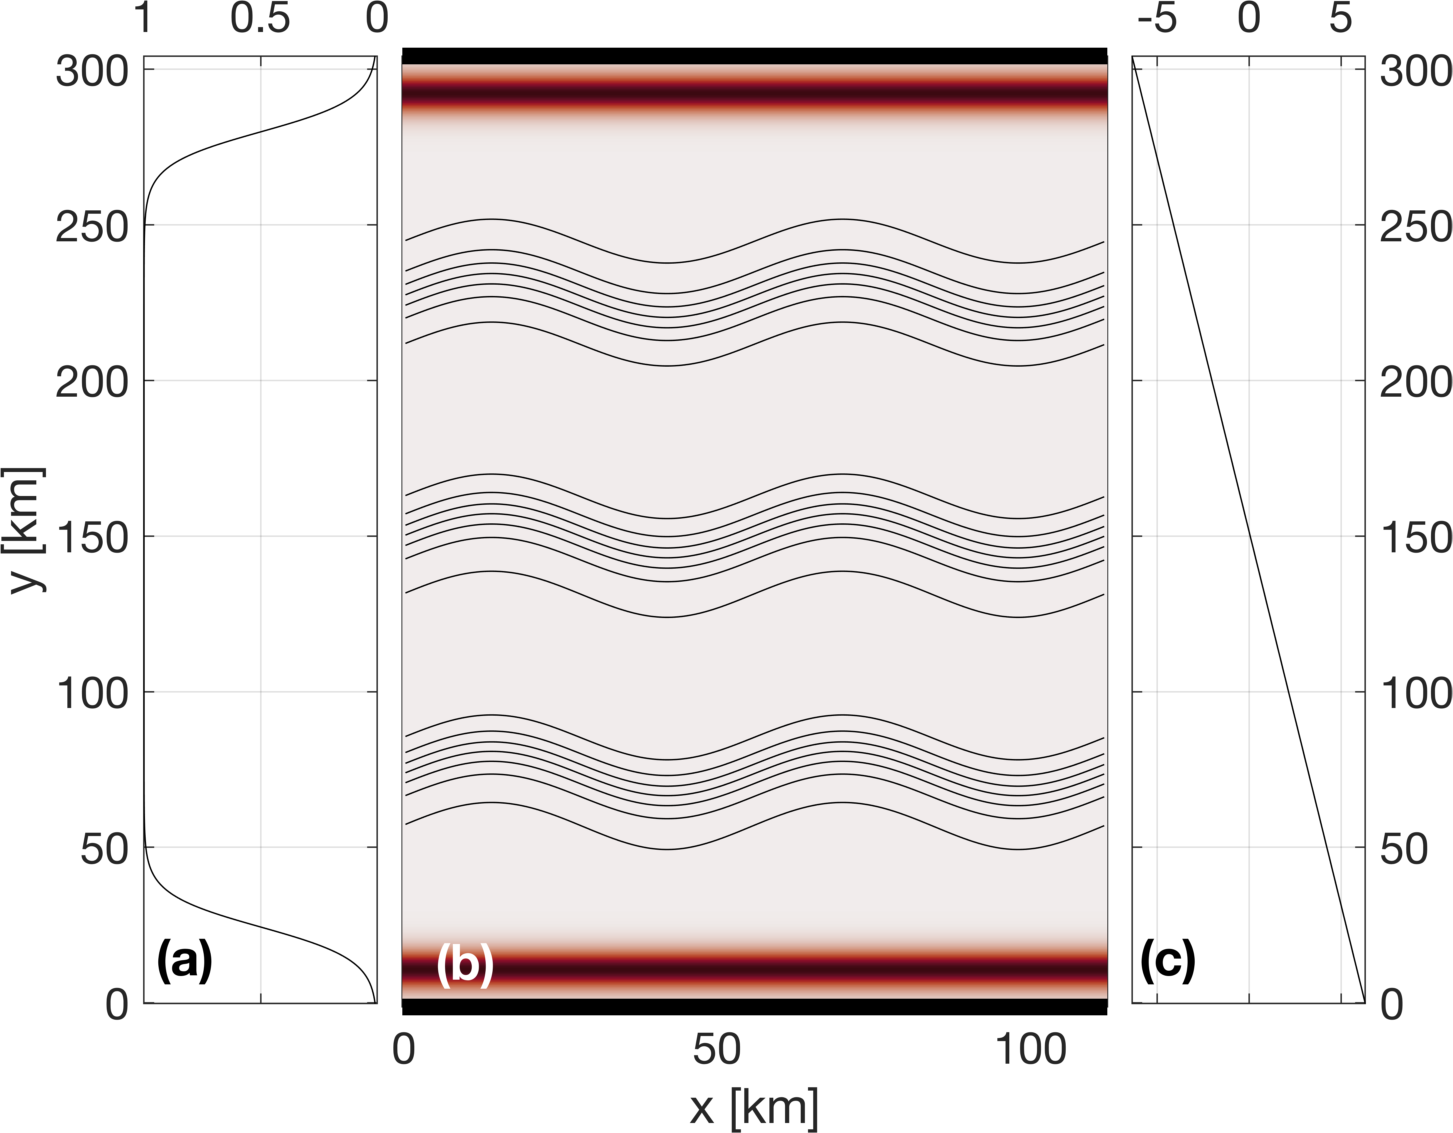
\includegraphics[width = .6\linewidth]{figures/Fig1_model_domain}
	\caption{PSOM model setup. (a) Meridional profile of zonal wind scaling coefficient that multiplies $\tau_x$, with a tapering at the north and south boundaries to reduce upwelling and downwelling, respectively. (b) Restoration factor (color shading) used to dampen internal wave reflection at boundaries as well as curl-driven upwelling and downwelling, along with constant density contours showing the three fronts (black line). (c) Surface net heat flux anomaly superimposed to the heat fluxes prescribed at $y = 150$ km.}
	\label{fig: model_domain}
\end{figure}

Time-varying wind stress and heat flux are prescribed at the surface boundary. Time series are computed from measurements collected at Station Papa and available through the Pacific Marine Environmental Laboratory\footnote{https://www.pmel.noaa.gov/ocs/Papa}. Climatologies of daily wind stress and net heat fluxes are calculated over the period 2007-2016 to produce a year-long time series. A squared low-pass filter with a cut-off frequency of 8.5 days is applied to both time series to remove high-frequency variability. In all numerical experiments, the simulations are first allowed to spin-down for the first 5 days with no forcing apply at the surface boundary. Surface wind stress and heat fluxes are then linearly ramped up between days 5 and 10 of the simulation, to reach realistic values at day 10. % (Figures \ref{fig: Papa_summer} and \ref{fig: Papa_winter}).
While the meriodional component, $\tau_y$, is set to zero, the zonal component of the wind stress, $\tau_x$, is prescribed at the surface throughout the model domain and is tapered at the northern and southern boundaries to avoid excessive Ekman-driven upwelling and downwelling that could contaminate the middle third of the model domain, where the analysis is focused (Figure \ref{fig: model_domain}a). A restoration time scale is prescribed to contain the curl-driven upwelling and downwelling regions generated by the tapering of the wind stress, as well as to limit internal wave reflection at the solid boundaries back into the domain (Figure \ref{fig: model_domain}b). Net surface heat fluxes are homogeneously prescribed throughout the domain, over which a linear meridional heat flux anomaly is superimposed to maintain a north-south gradient (Figure \ref{fig: model_domain}c). The flux anomaly is zero in the center of the domain, associated with the latitude of Station Papa, and has a meridional slope of 1/24 W/m$^2$/km, which was determined from the North American Regional Reanalysis (NARR) product \citep{Mesinger_2006}.

Initial hydrographic conditions are determined from a three-dimensional gridded field of temperature and salinity from ARGO floats \citep{Gaillard_2009,Gaillard_2016}. ARGO data is averaged monthly over the period 2002-2012 and two different months are used to initialize the two main numerical experiments for this study: Climatological conditions in April are used to initialize the \textit{Papa\_summer} experiment, while January climatological conditions are used to initialize the \textit{Papa\_winter} experiment (Table \ref{tab: meso_vs_submeso}). The north-south background density gradient is then intensified into three fronts located at $y = 75$, $y = 150$, and $y = 225$ km (Figure \ref{fig: model_domain}). The amplitude of the density gradient associated with the three fronts is determined from the probability distribution function (PDF) of the density gradients measured by underwater gliders deployed around Station Papa over the period 2008-2010 \citep{Pelland_2016}. To reduce model spin-up time, density fronts are perturbed by a sinusoidal wave with a wavelength close to the 1st baroclinic deformation radius ($\lambda = $ 66 km). Similar PSOM configurations were successfully used in previous studies \citep{Mahadevan_2012,Omand_2015}.

Two main experiments are conducted using the same configuration of PSOM, where only initial conditions and surface forcings are varied: \textit{Papa\_summer} aims at generating ocean dynamics mimicking conditions int the northeast Pacific in the summertime. Summer ocean dynamics are characterized by a flow generally in geostrophic balance, with relatively weak density gradients and low Rossby numbers ($\ll1$). \textit{Papa\_winter} aims at capturing wintertime ocean conditions in the region. A different dynamical regime is expected to dominate during wintertime, with submesoscale dynamics playing a more important role. Submesoscale dynamics are characterized by sharper density fronts, filament-like features and localized Rossby number $\mathcal{O}$(1) over spatial scales $\mathcal{O}$(1 km). Such dynamics are more likely to be found in the winter time, where mixed layers are deeper and lateral density gradients enhanced \citep{Thompson_2016}. The individual characteristics of each of \textit{Papa\_summer} and \textit{Papa\_winter} are detailed below.

\subsubsection{\textit{Papa\_summer} Model Experiment}

In \textit{Papa\_summer}, PSOM is initialized based on climatological ARGO data in April. The magnitude of the density gradient across the front (i.e., frontal sharpness) is set to 3.34$\times$10$^{-6}$ kg/m$^3$/m, which corresponds to the 95$^{th}$ percentile of the PDF of density gradients measured in April from glider data collected in the region (Figure \ref{fig: Papa_summer} and Table \ref{tab: meso_vs_submeso}). The model is run with a timestep of 216 s and is allowed to spin-up for 60 days, allowing summer stratification to develop. The model is then run for 30 additional days, saving instantaneous model fields every 3 hours for particle tracking. The month of April is chosen for initialization so the experiment would capture the onset of positive net heat fluxes, and the summer restratification that ensues in July-August (Figure \ref{fig: Papa_summer}). In this region, the summer stratification is associated with large primary productivity, particle production, and POC export \citep[e.g., fecal pallets, dead phytoplankter; ][]{Plant_2016}.

%TAB1
\begin{table}[t]
\caption{Summary of the key characteristics of PSOM experiments \textit{Papa\_summer} and \textit{Papa\_winter}.}
	\label{tab: meso_vs_submeso}
	\centering
 \centering
\begin{tabular}{|l|c|c|}
		\hline
											& \textit{Papa\_summer} & \textit{Papa\_winter} \\
		\hline
		Time period 								& April -- July             & January -- March          \\
		Spin-up								& 60 days                   & 50 days                   \\
		Advective timestep				    & 216 s                     & 108 s                     \\
		Horizontal diffusivity			    & 1 m$^2$/s                 & 0.2 m$^2$ s$^{-1}$        \\
		Restoration timescale			    & 3 days                    & 15 days                   \\
		Maximum M$^2$ ($\times$10$^{-8}$)	& 3.20 s$^{-2}$             & 33.9 s$^{-2}$             \\	
		Maximum N$^2$ ($\times$10$^{-4}$)	& 1.5 s$^{-2}$              & 1.6 s$^{-2}$              \\
		Initial mixed layer depth           & 73 m                      & 85 m                      \\
		Zonal wind stress                	& 0 -- 0.16 N m$^{-2}$      & -0.05 -- 0.17 N m$^{-2}$  \\	
		Surface heat flux               	& -46.8 -- 167.5 W m$^{-2}$ & -57.6 -- 15.3 W m$^{-2}$  \\	
		\hline
	\end{tabular}
\end{table}

% \begin{table}
% \caption{Time of the Transition Between Phase 1 and Phase 2$^{a}$}
% \centering
% \begin{tabular}{l c}
% \hline
%  Run  & Time (min)  \\
% \hline
%   $l1$  & 260   \\
%   $l2$  & 300   \\
%   $l3$  & 340   \\
%   $h1$  & 270   \\
%   $h2$  & 250   \\
%   $h3$  & 380   \\
%   $r1$  & 370   \\
%   $r2$  & 390   \\
% \hline
% \multicolumn{2}{l}{$^{a}$Footnote text here.}
% \end{tabular}
% \end{table}


% FIG2
\begin{figure}[t]
	\includegraphics[width = 1\linewidth]{figures/Fig2_Papa500_summer}
	\caption{PSOM configuration for \textit{Papa\_summer}. (a) Time series of net heat fluxes and wind stress prescribed at the surface. Notice the positive heat fluxes, as well as downfront winds (i.e. eastward) persisting throughout the experiment. (b)-(d) horizontal buoyancy gradients $M^2 = |\nabla_Hb|^2$ (in s$^{-2}$) at day of year (doy) 105, 135, and 165. Black contours show isopycnals (in kg/m$^3$; CI = 0.01 kg/m$^3$). (e) Vertical profile of the buoyancy frequency $N^2$ at doy 105, 135, 165, and 195, showing the development of summer stratification centered at z = 30 m (solid lines). Monthly-average vertical stratification obtained from glider profiles collected in June and July are superimposed (dashed lines), along with the correlation coefficient between observations and model outputs.}
	\label{fig: Papa_summer}
\end{figure} 


\subsubsection{\textit{Papa\_winter} Model Experiment}

In \textit{Papa\_winter}, PSOM is initialized based on climatological ARGO data in January. The frontal sharpness is set to 3.54$\times$10$^{-5}$ kg/m$^3$/m, which corresponds to the 99$^{th}$ percentile of the PDF of density gradients measured in January from glider data collected in the region (Figure \ref{fig: Papa_winter} and Table \ref{tab: meso_vs_submeso}). The model is allowed to spin-up for 50 days allowing for the prescribed fronts to become unstable. To accommodate the larger density gradients, the advective timestep is shortened to 108 s, and the horizontal diffusivity is lowered to 0.2 m$^2$/s. The model is run for 30 additional days, saving instantaneous model fields every 1.5 hours for particle tracking. The month of January is chosen for initialization so the experiment would capture the time of year where the mixed layer is the deepest, and Rossby number of O(1) are more likely to occur. The objective is for this experiment to contrast \textit{Papa\_summer} by capturing the statistics of ocean conditions dominated by submesoscale dynamics.

% FIG3
\begin{figure}[ht]
	\includegraphics[width = 1\linewidth]{figures/Fig3_Papa500_winter}
	\caption{PSOM configuration for \textit{Papa\_winter}. (a) time series of net heat fluxes and wind stress prescribed at the surface. Notice the mostly negative heat fluxes, as well as alternating zonal wind direction. (b)-(d) horizontal buoyancy gradients $M^2 = |\nabla_Hb|^2$ (in s$^{-2}$) at day of year (doy) 0, 30, and 50. Black contours show isopycnals (in kg/m$^3$; CI = 0.01 kg/m$^3$). (e) Vertical profile of the buoyancy frequency $N^2$ at doy 0, 30, 50, and 80, showing the persistence of the halocline between z = 80 and z =180 m throughout the experiment (solid lines). Monthly-average vertical stratification obtained from glider profiles collected in March is superimposed (dashed line), along with the correlation coefficient between observations and model outputs.}
	\label{fig: Papa_winter}
\end{figure}


\subsubsection{Validation}
\label{sec: glider_validation}

To ensure that PSOM simulations yielded realistic conditions for both \textit{Papa\_summer} and \textit{Papa\_winter}, distributions of horizontal ($M^2$) and vertical ($N^2$) buoyancy gradients are compared with glider observations collected over the period 2008-2009 \citep{Pelland_2016}.

During this period, underwater gliders sampled in a ``bow-tie" pattern centered on Station Papa. Gliders sample the water column following a triangular wave, whose shape is easily affected by currents, due to the slow moving speed of the glider ($\sim$1 km/hr). It is therefore challenging to associate a specific spatial scale with gradients computed between glider profiles, as profile separation distances can be highly variable through depth and time. To circumvent this issue, horizontal buoyancy gradients are computed between each pair of glider profiles available within one branch of the bow-tie. Each along-track buoyancy gradient is then associated with a separation scale and a timestamp. 

 Glider-based density gradients are highly affected by internal waves. To filter the impact of internal waves on the PDF of horizontal buoyancy gradients, only gradients computed at a scale of $\pm$ 1 km of twice the Rossby radius are considered. Rossby radii are $\sim 8$ km in winter and $\sim 20$ km in summer.
 
\subsection{Particle Tracking Experiments}

\subsubsection{Particle Advective Scheme}
To quantify the impact of submesoscale dynamics on the export of Particulate Organic Matter (POC), Lagrangian particle tracking is used in conjunction with the flow field obtained from the two experiments described above. Particles are tracked using the non-divergent velocity field at each face of a grid cell. The velocity field is then linearly interpolated onto the particle's position. For example, the eastward velocity (x-axis) of a particle is given by:

\begin{equation}
u(x) = u_{i-1} + \frac{(x - x_{i-1})}{(x_i - x_{i-1})}(u_{i}-u_{i-1})
\end{equation}
where the subscripts $i-1$ and $i$ denote the western and eastern walls of the grid cell where the particle is located, respectively. This can be re-written as:

\begin{equation}
\frac{\partial x}{\partial t} + \beta x + \delta =  0
\label{eq: eq_diff}
\end{equation}
where $\beta = (u_{i}-u_{i-1})/\Delta x$ and $\delta = -u_{i-1} - \beta x_{i-1}$ \citep{Doos_2013}. This differential equation can be solved analytically for $\beta \neq 0$:

\begin{equation}
x_{t_1} = \left(x_0 + \frac{\delta}{\beta}\right)\exp^{-\beta(t_1 - t_0)} - \frac{\delta}{\beta}
\label{eq: PT_advection}
\end{equation}
The time it will take for the particle to reach the eastern or western face of the grid cell can be computed by taking $x_{t_1} = x_i$ or $x_{t_1} = x_{i-1}$, respectively, and solving for $t_1$. For each advective timestep, the times required for the particle to reach any of the 6 walls of the grid cell are computed using Equation \ref{eq: PT_advection}. If any of those times is shorter than the advective timestep, the particle is advected until it reaches the cell wall. Then the flow field in the adjacent grid cell is considered and the particle is advected over the remaining time. For each particle tracking experiment, four different classes of particles were released. Each particle class is characterized by a different sinking velocity: 0.025, 0.05, 1, and 5 m/day. The slowest-sinking class was essentially selected to represent non-sinking particles: based on the setup of our experiments, the slowest-sinking particles would take 800 days on average to be exported through gravitational sinking, a timescale much greater than commonly observed remineralization timescales. The fastest-sinking velocity is chosen as a low end-member representing velocity classes that will be exported in its entirety over the course of our experiment. The results presented for the 5 m/day sinking class can therefore be extrapolated to any class with a higher sinking velocity. 

In the horizontal, particles are seeded once every 250 m over the entire domain in the x-direction, and for 100 $<y<$ 200 km in the y-direction. The seeding is centered on the position of the middle front (see Figure \ref{fig: Papa_summer}) and is therefore not affected by artificial features developing at the solid north and south boundaries. In the vertical, eleven of those sheets of particles are seeded every 1 m between 75 and 85 m. This depth range is chosen as it corresponds to the average euphotic depth at Station Papa, defined as the 1\% light level. The euphotic depth was computed for the months of February and June over the period 2007-2016 from profiles of Photosynthetically Available Radiation (PAR) collected at Station Papa as part of the long-term monitoring of Line P executed by the Department of Fisheries and Ocean Canada\footnote{https://www.waterproperties.ca/linep/index.php}. The average euphotic depth computed for both of these months is around 80 m, which agrees with previously established estimates of the euphotic depth \citep{Sherry_1999,Harrison_2004}.

The particle advective timestep is set to 1.5 hours. The flow field is linearly interpolated in time between model outputs, justifying the higher temporal resolution used for particle tracking in \textit{Papa\_winter}. Particle positions are saved every 3 hours, along with key model variables interpolated onto the particle positions (e.g., density, vorticity). Particles are tracked for three weeks (28 days). Each particle-tracking experiment contains 1,971,717 particles per sinking-velocity class, for a total of 9,858,585 particles. Particles located deeper that the maximum winter mixed layer \citep[i.e., 100 m;]{Pelland_2016, Plant_2016} are considered exported, as they will likely not be re-suspended into the mixed layer. %The export horizon is therefore set to 100 m, based on the seasonal cycle observed at Station Papa \citep{Pelland_2016}.

\subsubsection{Density and Biomass Spectra}
\label{sec: equations_biomass}
The slope of the size spectrum of particles is traditionally described by the slope of the log-log curve, $\xi$, between particle number $N$ and particle radius $r$ \citep[also know as the Junge slope;][]{White_2015}:

\begin{equation}
N(r) = N_0 \left(\frac{r}{r_0}\right)^{-\xi}
\label{eq: powerlaw_radius}
\end{equation}
where $N_0$ and $r_0$ represent a reference particle number and radius, and are chosen arbitrarily. For small particles ($<400\mu m$) and relatively cold temperature ($<15^oC$), it has been shown that the relationship between particle radius $r$ and sinking velocity $w_s$ tend to follow Stokes law, with $w_s \propto r^2$ \citep{Bach_2012}. \cite{Bach_2012} also demonstrates that Stokes law is generally a lower-bound limit to estimate sinking velocities for a specific particle size. Assuming a Stokes-like relationship, Equation \ref{eq: powerlaw_radius} can thus be re-written in terms of sinking velocities:

\begin{equation}
N(w_s) = N_0 \left(\frac{w_s}{w_{s_0}}\right)^{-\xi/2}
\label{eq: powerlaw_velocity}
\end{equation}
For a specific slope and sinking-velocity class, an equivalent number of particles per simulated particle can thus be computed using Equation \ref{eq: powerlaw_velocity} (See Figure \ref{fig: sinking_velocity_spectrum}). For example, using the largest sinking velocity class as a reference (i,.e., $w_{s_0} = 5$ m/day and $N_0=$1,971,717), and a spectral slope $\xi = 4$, each simulated particle with a sinking velocity of 0.025 m/day in fact represent 40,000 particles (Figure \ref{fig: sinking_velocity_spectrum}). The relative biomass of a particle in a specific sinking-velocity class, $B_p(w_s)$, can be estimated if the biomass is assumed to vary with the particle's volume. The relative biomass of one particle in a sinking-velocity class $w_s$ can therefore be computed using:

% FIG4
\begin{figure}[ht]
	\centering
	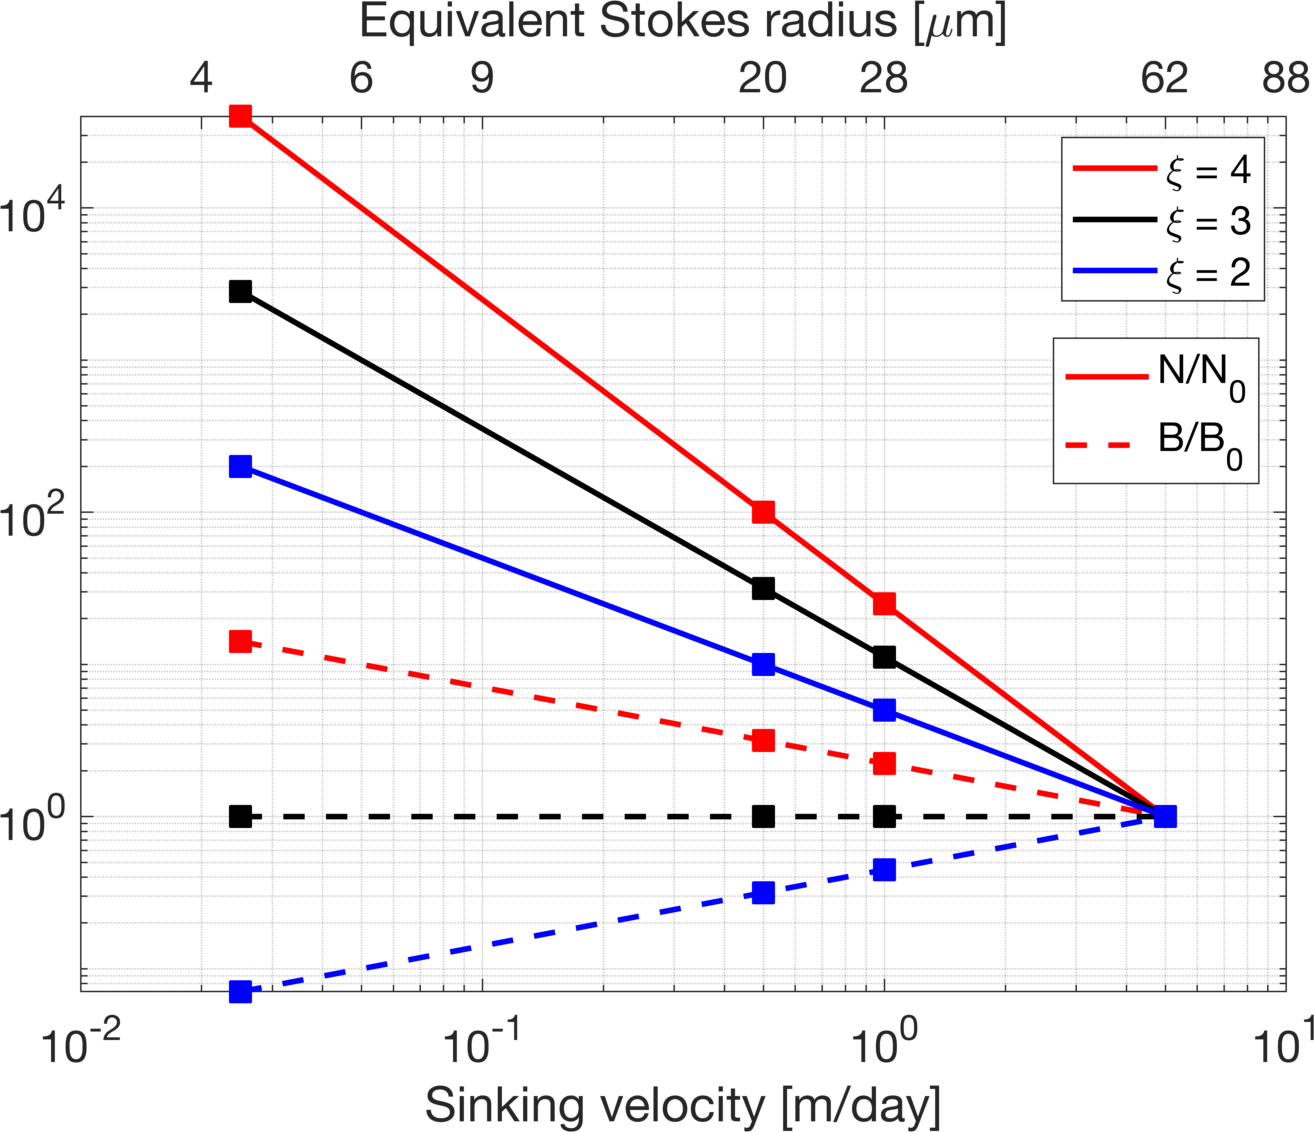
\includegraphics[width = .6\linewidth]{figures/Fig4_particle_PDF}
	\caption{Normalized number of particles (solid) and biomass (dashed) to the fastest-sinking particle class. Sinking velocity spectrum are shown for three different Junge slope $\xi$: 4 (red), 0 (black), and 2 (blue).}
	\label{fig: sinking_velocity_spectrum}
\end{figure}

\begin{equation}
	B_p(w_s) = B_p(w_{s_0})\left(\frac{w_s}{w_{s_0}}\right)^{3/2}
	\label{eq: biomass_realparticle}
\end{equation}
where $B_p(w_{s_0})$ is a reference biomass of one particle in the sinking velocity class $w_{s_0}$. The total biomass associated with one simulated particle can be obtained by scaling Equation \ref{eq: biomass_realparticle} by the ratio $N(w_s)/N_0$:

\begin{equation}
	B(w_s) =  B_0\left(\frac{w_s}{w_{s_0}}\right)^{3/2}\frac{N(w_s)}{N_0}
	\label{eq: biomass_simulatedparticle}
\end{equation}
where $B_0 = B_p(w_{s_0})$. Combining Equations \ref{eq: powerlaw_velocity} and \ref{eq: biomass_simulatedparticle} yields an expression relating the biomass associated with a simulated particle for a specific sinking-velocity class and the spectral slope (Figure \ref{fig: sinking_velocity_spectrum}):
\begin{equation}
	B(w_s) = B_0\left(\frac{w_s}{w_{s_0}}\right)^{\frac{3-\xi}{2}}
	\label{eq: biomassjungeslope}
\end{equation}
Using the same example as before where $\xi = 4$, if the amount of biomass associated with one simulated particle in the 5 m/day sinking-velocity class is taken as $B_0 = 1$, then one simulated particle sinking at 0.025 m/day contains 14.14 units of biomass and a single particle contains $14.14/40,000 =3.5\times10^{-4}$ units of biomass (see Figure \ref{fig: sinking_velocity_spectrum}). This normalized formulation of particle number and biomass (Equations \ref{eq: powerlaw_velocity} and \ref{eq: biomassjungeslope}) presents the advantage that the impact of spectral slope on the relative export of biomass can be quantified without needing a large number of particle-tracking experiments. For the purpose of this study, only the relative amount of biomass is relevant. For simplicity, we therefore define a normalized biomass unit as $B_0=$ 1.

\subsubsection{Particle Remineralization Scheme}
\label{sec: remin_scheme}
Remineralization of particles as they sink through the water column evidently impact the export of biomass. Slow-sinking particles therefore are subject to shallower remineralization than fast-sinking particles. In this study, the impact of remineralization is considered through the implementation of a time-dependent sinking velocity. Remineralization processes driving remineralization rates are complex, species-dependent, and generally not well-understood. In the absence of a consensus on a general functional form of particle remineralization, we rely on an idealized relationship linking carbon content and time. This implicitly assumes that the biomass content of a particle diminishes in time proportionally to the particle volume. Remineralization is thus modeled as an exponential decrease of biomass with time at a rate $k$ \citep{Iversen_2010, Iversen_2013}:
\begin{equation}
	B (t) = B^0\exp(-kt)
	\label{eq: remin_scheme}
\end{equation}
where $B^0$ denotes the biomass content at $t = 0$ days, and $k = 0.13$ day$^{-1}$. This remineralization rate determined by \cite{Iversen_2010} is independent of particle sinking velocity, and seems to generally agree with other findings, despite the large uncertainties \citep{Ploug_2008, Iversen_2013}. The change in biomass with time is in turn expected to affect the sinking velocity of the particle. Given that $B \propto w^{3/2}$ (see Equation \ref{eq: biomass_realparticle}),  a time-varying sinking velocity is imposed to particles in all sinking-velocity classes using:

\begin{equation}
w_s (t) = w_s^0\exp(-\frac{2kt}{3})
\label{eq: sinking_velocity_remin}
\end{equation}
where $w_s^0$ is the initial sinking velocity at $t = 0$ days. Particles are classified based on their initial sinking-velocity. However, it is worth noting that over the length of the particle-tracking experiments including remineralization (28 days), particles slow down by more than 90\% of their initial velocity.

\section{Results}
\label{sec: Results}
\subsection{Physical model}

Two model experiments are designed to capture different dynamical conditions observed in the northeast Pacific Ocean in summer and winter. \textit{Papa\_summer} is initialized in early spring (doy 105) when the water column is characterized by a relatively deep mixed layer ($\sim$100 m) and a halocline present between 100 and 150 m (Figure \ref{fig: Papa_summer}). The forcing by a realistic, positive, net heat flux generates the restratification of the water column, with the development of a strong thermocline between 25 and 50 m leading to the shoaling of the mixed layer and a subsurface peak in $N^2$ at about 30 m (see Figure \ref{fig: Papa_summer}). A comparison between model outputs and monthly-averaged density profiles from underwater gliders collected in June and July over the period 2008-2009 yields correlation coefficients of $r = 0.87$ and $r = 0.88$, respectively. These correlation coefficients suggest that \textit{Papa\_summer} captures reasonably well the vertical spring and summer conditions in the northeast Pacific Ocean.

In the horizontal, the prescribed density fronts progressively become unstable within the first 60 days of the experiment (Figure \ref{fig: Papa_summer}). During this time, the Total Kinetic Energy (TKE) contained in the model domain slowly increases before reaching a maximum at doy 162, where it remains relatively constant for the rest of the simulation. The flattening of the TKE curve is used to determine the time necessary for the simulation to spin-up, hence determining the start day of the particle-tracking experiments. The ocean dynamics associated with \textit{Papa\_summer} are characterized using PDFs of horizontal buoyancy gradients ($M^2 = |\nabla_Hb|^2$), vertical velocities ($w$), and Rossby numbers computed from the normalized vertical component of the relative vorticity (Ro $=( \partial v/ \partial x - \partial u/ \partial y)/f$; Figure \ref{fig: dynamics}).

%FIG5
\begin{figure}[t]
	\centering
	\includegraphics[width = 1\linewidth]{figures/Fig5_dynamic_signature_w_valid}
	\caption{Snapshots of $M^2$ (top), $\zeta /f$ (middle), and $w$ (bottom) half-way through the particle tracking experiment for \textit{Papa\_summer} (left and blue) and \textit{Papa\_winter} (right and red), with the Mixed Layer Depth indicated by the solid black line. The corresponding Probability Distribution Functions (PDFs) are shown in the center. Note the changing color scales between \textit{Papa\_summer} and \textit{Papa\_winter}. Histograms of M$^2$ computed from glider data at Station Papa in February (blue line) and July (red line) are superimposed in the top middle panel.}
	\label{fig: dynamics}
\end{figure}

The largest horizontal buoyancy gradients are observed above the thermocline ($z<$50 m) and along the halocline (100-200 m), and range between 0 and 1.2$\times 10^{-7}$ s$^{-2}$ (Figure \ref{fig: dynamics}). These relatively weak density gradients result in low Rossby numbers O(0.1), positive on the denser (north) side of the front, and negative on the lighter (south) side of the front. Corresponding vertical velocities are consistently weaker than 1 m/day ($<$10$^{-5}$ m/s) and are characterized by regions of weak upwelling and downwelling on the order of 10 km, associated with the meandering of the front \citep{Bower_1989}. Alternating bands of upwelling and downwelling at $\mathcal{O}$(1 km) spatial scale are superimposed, likely caused by propagating internal waves. Coherent vertical velocities structures are homogeneous to depths much greater than the mixed layer depth ($\sim$25 m; Figure \ref{fig: Papa_summer}). The amplitude of the vertical velocity field coincides with the expected order of magnitude given by the scaling $w \propto RofU/N$ \citep{Mahadevan_2016}: using $Ro\sim0.1$ (Figure \ref{fig: dynamics}), $N\sim10^{-2}$ 1/s (Figure \ref{fig: Papa_summer}), $f\sim10^{-5}$ 1/s, and $U\sim0.01$ m/s, we obtain $w\sim 10^{-6}$ m/s. The agreement between the scaling and the model outputs suggest that PSOM is capable of reproducing a realistic vertical flow field.

\textit{Papa\_winter} is, on the other hand, initialized in the winter (doy 0) with the objective to capture a time period where the mixed layer depth is deeper ($\sim$ 100 m) and density gradients more pronounced \citep{Pelland_2016}. At this time of year, the water column in this region is characterized by the presence of a deep halocline between 100 and 150 m. After spin-up, the vertical stratification remains consistent throughout the model run, and compares well to the vertical profile obtained from glider observations for the month of March ($r = 0.95$; see Figure \ref{fig: Papa_winter}). In the horizontal, prescribed density fronts are much sharper than in \textit{Papa\_summer} (O(1 km ) vs. O(10 km)). Because of these stronger density gradients, combined with the alternating zonal winds and constantly negative surface heat flux, the fronts become unstable more rapidly than in \textit{Papa\_summer} (Figure \ref{fig: Papa_winter}). As a result, TKE starts to plateau at doy 48. The experiment is considered spun-up by doy 50 and the particle-tracking experiment is initialized. %Many sharp fronts and filaments on the order of 1 km can be seen in \textit{Papa\_winter}, penetrating to ocean upper layer to the deeper than in the summer, dissipating within the mixed layer at $\sim$100 m (Figure \ref{fig: dynamics}). 

The frontal structures visible in the horizontal buoyancy gradient field are logically associated with filaments of relatively high Rossby numbers, regularly exceeding O(1) (Figure \ref{fig: Papa_winter}). The PDF of Rossby numbers reveals a positively-skewed distribution of Rossby numbers ($s = 0.68$). This is in agreement with the fact the relative vorticity is more likely to be cyclonic than anticyclonic, based on conservation of potential vorticity \citep{Hoskins_1972}. Regions with a high Rossby number are localized and located in the mixed layer exclusively. In places where the local Rossby number reaches O(1), geostrophic balance is lost and a vertical secondary ageostrophic circulation develops to slump the isopycnals and return to a more stable geostrophically-driven flow. This ageostrophic secondary circulation therefore generates ``hot spots" of higher vertical velocities. The fine-scale structures in the vertical velocity field corresponding to Rossby numbers O(1) can be seen in Figure \ref{fig: Papa_winter}, with local vertical velocities up to 60 m/day ($\sim 7\times10^{-4}$ m/s; Figure \ref{fig: dynamics}). Contrarily to the PDF of Rossby numbers, the distribution of vertical velocities demonstrate a negative skewness ($s =$ -0.25). This is in agreement with the theory: In fact, positive vertical vorticity is associated with the dense side of a density front, where Rossby numbers are positive and vertical velocities negative \citep{Mahadevan_2016}. Once again, the amplitude of these vertical velocity hot spots is coherent with the scaling $w \propto RofU/N$: using $Ro\sim1$, $N\sim10^{-2}$ 1/s, $f\sim10^{-5}$ 1/s, and $U\sim0.1$ m/s, we obtain $w\sim 10^{-4}$ m/s. This demonstrates the capabilities of PSOM to resolve sharp frontal features at the kilometer scale, as well as the ageostrophic circulation associated with those fronts. 

Comparing \textit{Papa\_summer} and \textit{Papa\_winter} highlights the different dynamical regimes in the two experiments. In \textit{Papa\_winter}, density fronts tend to be sharper, meaning larger density gradients over shorter spatial scales. When computed at the kilometer-scale, the PDF of horizontal buoyancy gradients in \textit{Papa\_winter} exhibits a longer tail than in \textit{Papa\_summer} (Figure \ref{fig: dynamics}). When compared to observations, the PDFs of $M^2$ in \textit{Papa\_summer} and \textit{Papa\_winter} demonstrate a correlation with observations of $r = 0.93$ and $r = 0.95$, respectively


The wider PDF of vertical velocities in \textit{Papa\_winter} shows advective velocities that match and exceed typical gravitational sinking velocities, particularly for smaller, and therefore slower-sinking, particulate organic material. The secondary ageostrophic circulation that develops at submeso-scales (i.e., Ro O(1)) therefore generates an export mechanism that directly competes with the traditional paradigm that relies on gravitational sinking leading the export of particulate matter in the ocean.

\subsection{Particle tracking}

Both model experiments described above were then used to investigate the relationship between ocean dynamics and particle export, using Lagrangian particle-tracking. In this study, particles are considered "exported" once located below the depth of the winter mixed layer, which roughly corresponds to the 100 m depth horizon at Station Papa. Choosing the winter mixed layer as the export depth is most appropriate, as it reduces the chances of particles being re-entrained into the mixed layer the following winter. We first consider the case of conservatives particles that do not remineralize in order to better identify the effects of ocean dynamics and spectral slope on export.

The percentage of simulated particles being exported with time is shown in Figure \ref{fig: particle_export} for both \textit{Papa\_summer} and \textit{Papa\_winter}. As expected, the faster-sinking particles are exported earlier and in larger proportions. For \textit{Papa\_summer} specifically, only the two fastest sinking-velocity classes (5 and 1 m/day) are exported within the first 28 days, while the other sinking-velocity classes do not significantly export particles over this time period ($<$ 5\%). In fact, time series of exported particles closely follow the curves derived from considering gravitational sinking only (Figure \ref{fig: particle_export}).

%FIG6
\begin{figure}[ht]
	\centering
	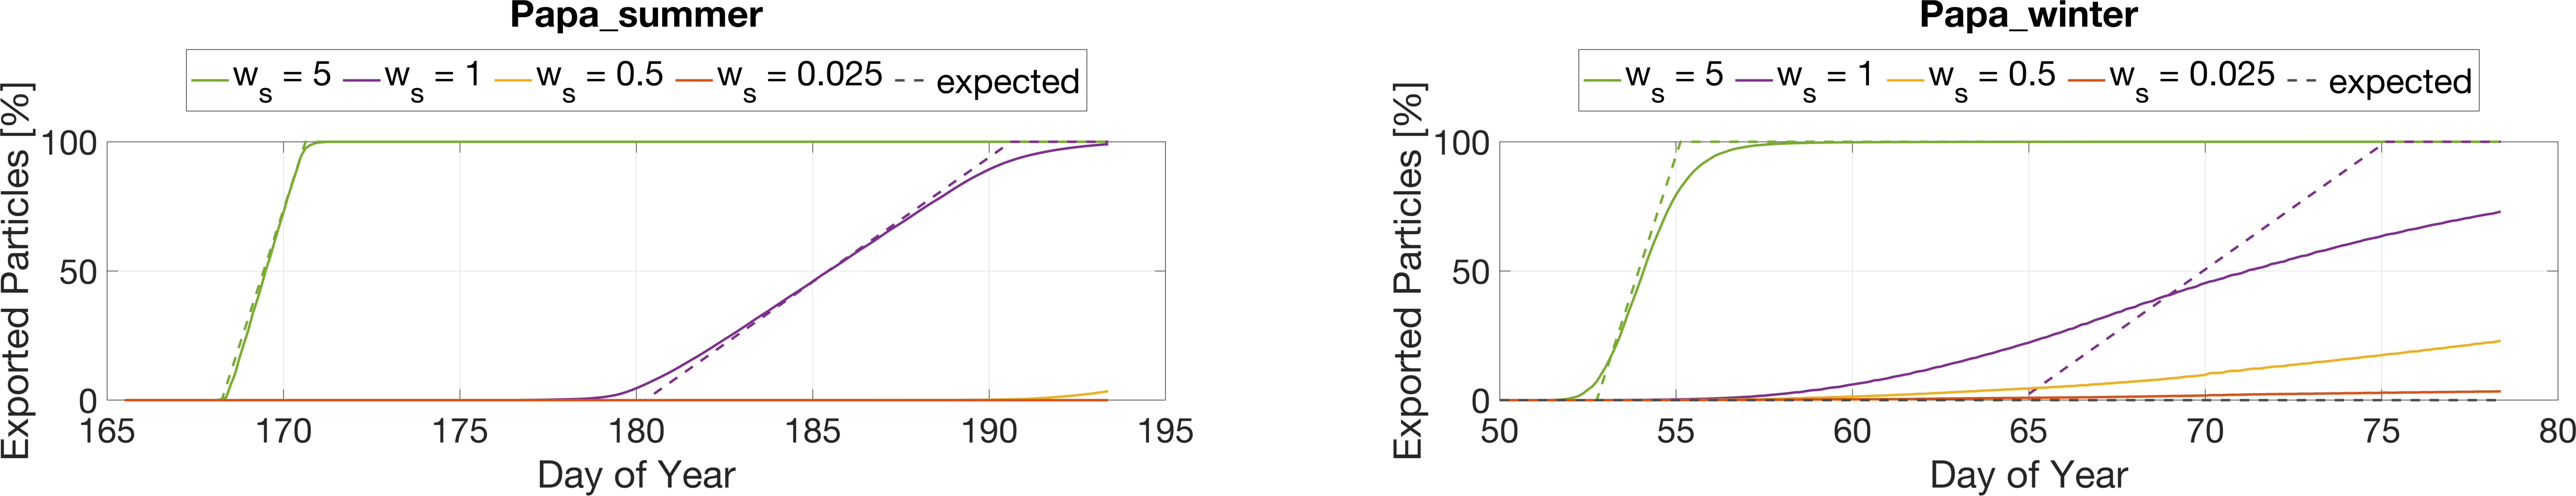
\includegraphics[width = 1\linewidth]{figures/Fig6_particle_export}
	\caption{Percentage of particles located below 100 m as a function of time in \textit{Papa\_summer} (left), and \textit{Papa\_winter} (right). Expected percentages of exported particles based on gravitational sinking only are indicated with dashed lines.}
	\label{fig: particle_export}
\end{figure}

Time series of exported particles in \textit{Papa\_winter} present major differences. In every sinking-velocity class, particles reach the export depth faster than expected from gravitational sinking. This early arrival of particles is accentuated as the sinking-velocity decreases, ranging from about 1 day early for particles sinking at 5 m/day, to about 10 days early for particles sinking at a rate of 1 m/day. Sinking-velocity classes that are not expected to reach the export depth within the first 28 days now significantly contribute to export within the first 15 days of the simulation. Over 20\% of particles sinking at 0.5 m/day is now exported, versus less than 5\% in \textit{Papa\_summer}. About 5\% of particles sinking at 0.025 m/day are exported. However, more time is now necessary to export 100\% of the simulated particles. This can be seen in the gentler slopes of the export curves observed in \textit{Papa\_winter} than in \textit{Papa\_summer}.

Particles released in \textit{Papa\_winter} are thus exported faster and in greater number than expected from gravitational sinking only. Eventually, all sinking particles would be exported in both \textit{Papa\_summer} and \textit{Papa\_winter}, if particles were tracked for a long enough period of time. Particles, and specifically slow-sinking ones, are however expected to remineralize on timescales shorter than their export timescale. The impacts of remineralization on export are presented and discussed in Sections \ref{sec: results_remin} and \ref{sec: discussion_particle}.

The presence of submesoscale dynamics therefore increases the number of exported slow-sinking simulated particles, by anywhere between a few percent and tens of percents, depending on the sinking-velocity class. This has large implications on the amount of biomass exported, as slower-sinking particles are far more numerous than faster-sinking particles, despite containing less biomass (Figure \ref{fig: sinking_velocity_spectrum}). While the number of simulated particles that are exported is only a function of the modeled flow field, the exported biomass also depends on the Junge slope (see Equation \ref{eq: biomassjungeslope}).

The impact of ocean dynamics on the respective contributions of the different sinking velocity classes to the total exported biomass is fairly intuitive: For a specific Junge slope, the presence of submesoscale dynamics enhance the role played by slower-sinking particles in biomass export, and thus decrease the importance of faster-sinking particles (Figure \ref{fig: biomass_export_remin}). This is a logical results in sight of the increase in the number of particles exported when submesoscales features are present (Figure \ref{fig: particle_export}). The sinking class dominating export, however, is highly dependent on the Junge slope parameter. As the Junge slope parameter increases, the particle spectrum steepens, and the contribution of slower-sinking particles to the total exported biomass increases, sometimes dominating biomass export. For example, after 28 days, the 1 m/day exports 50\%, 100\%, and 125\% of the biomass exported by the 5 m/day class when $\xi =$ 2, 3, and 4, respectively.

%FIG7
 \begin{figure}[ht]
	\centering
	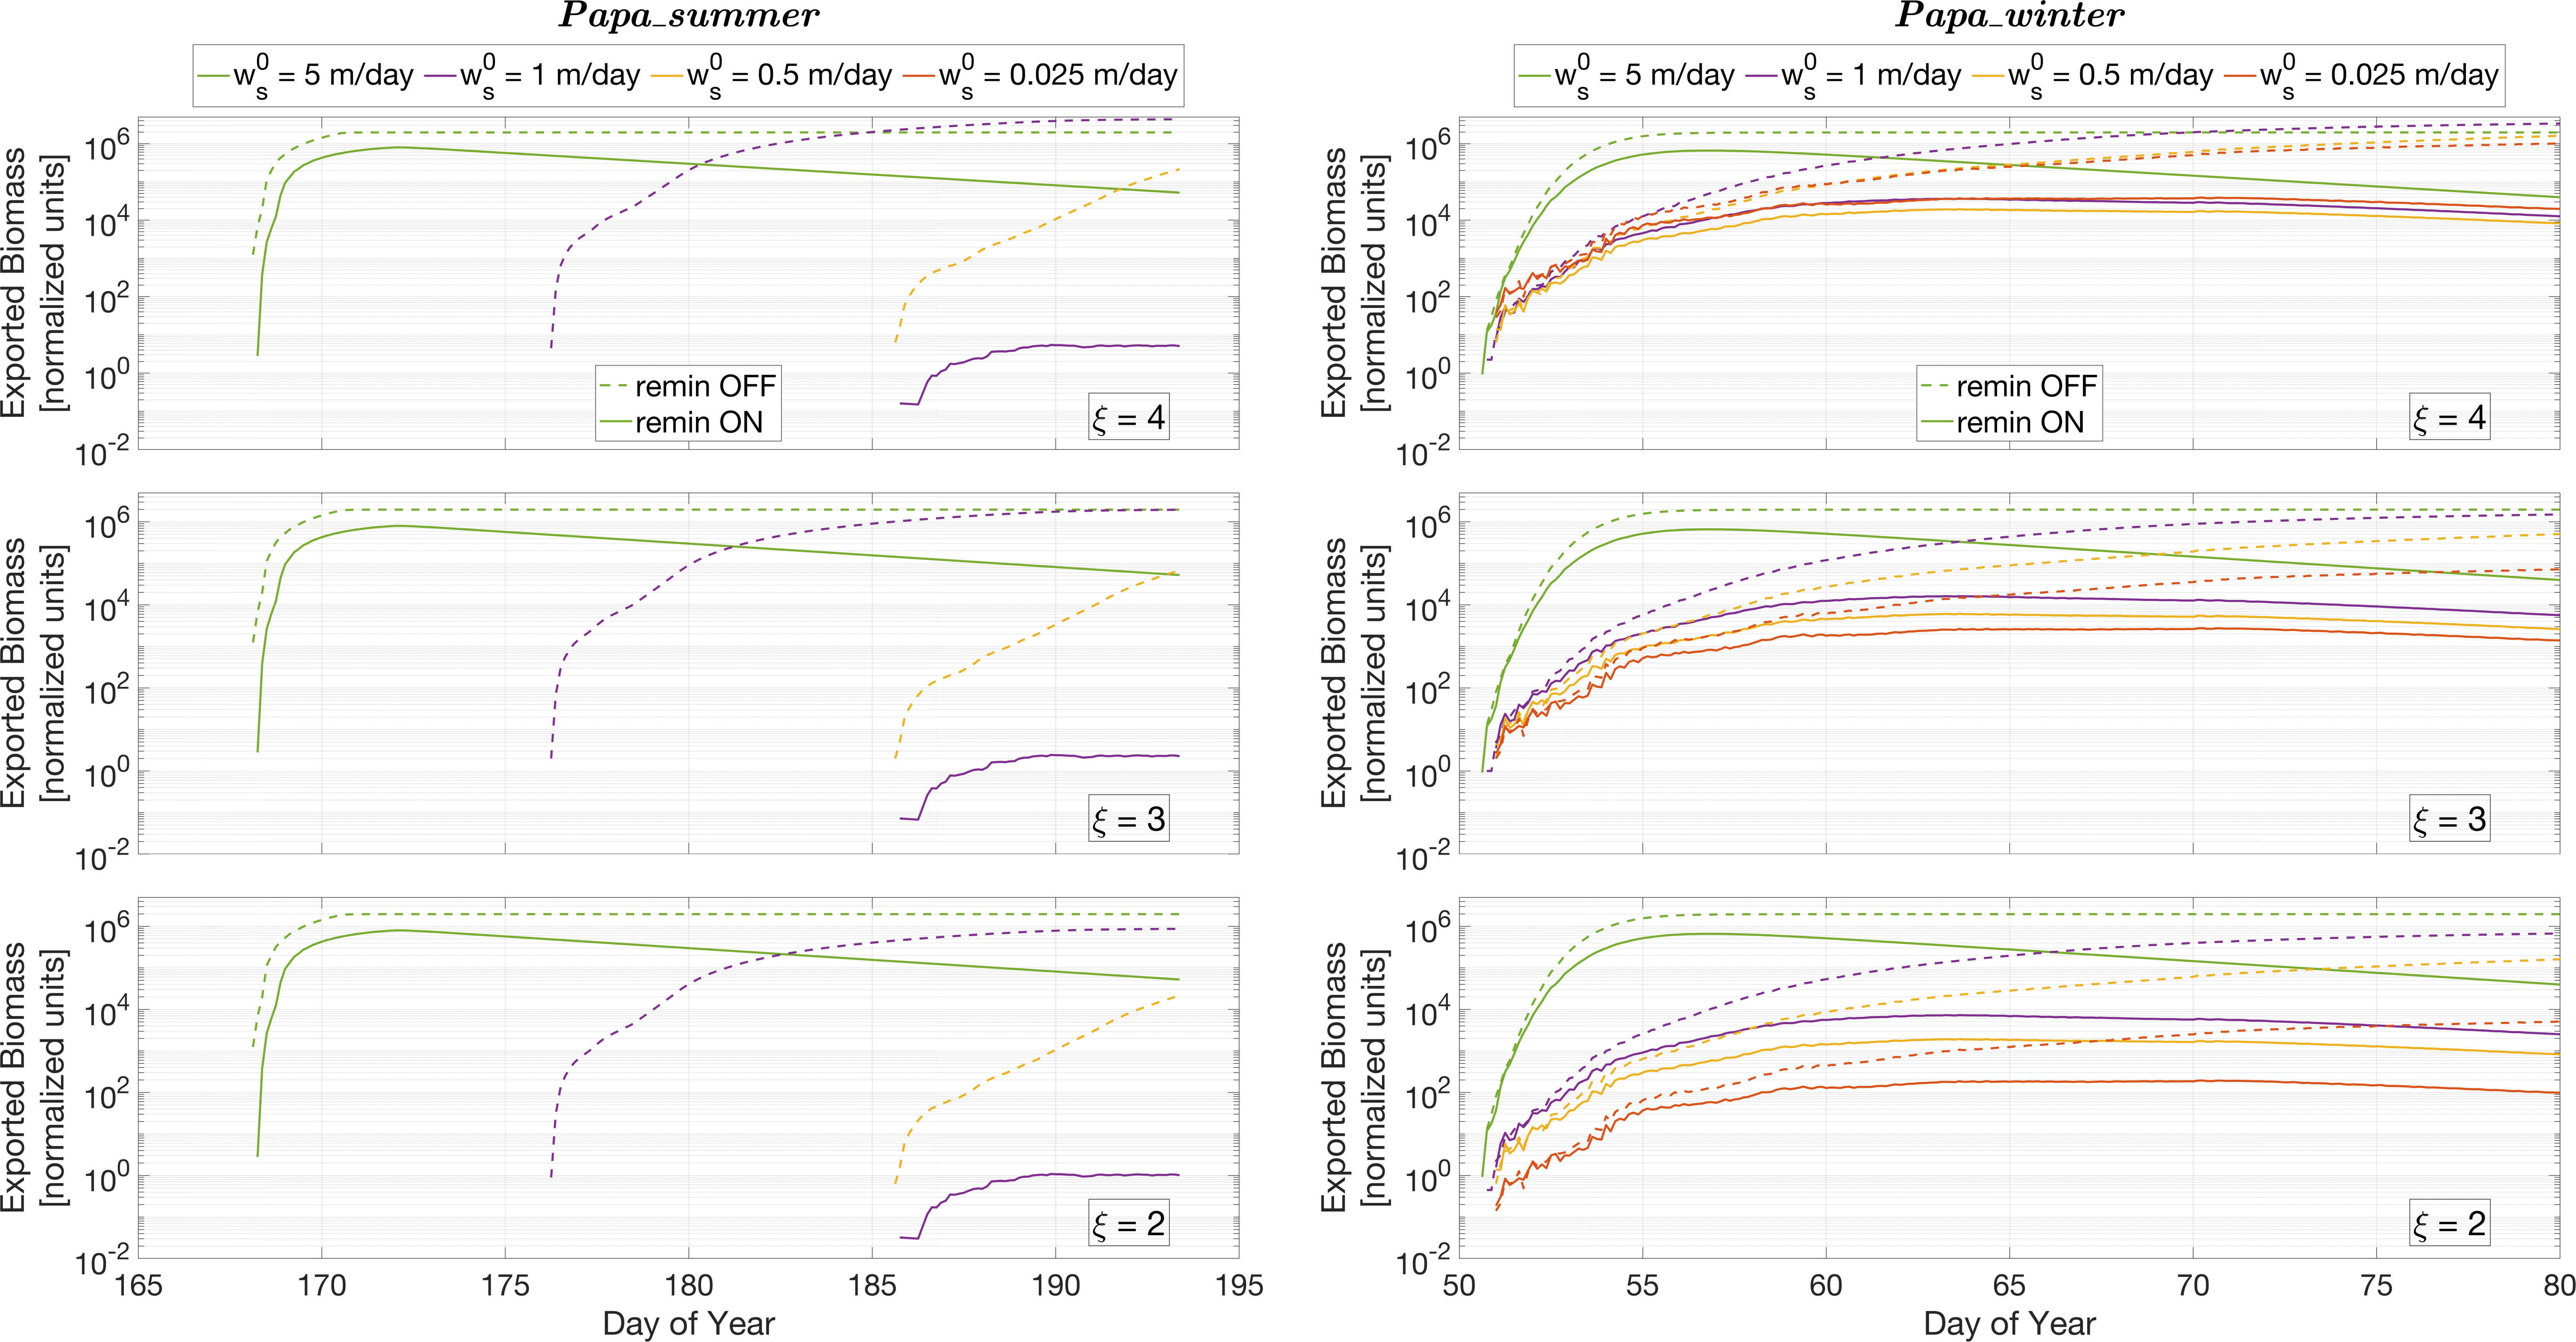
\includegraphics[width = 1\linewidth]{figures/Fig7_biomass_export}
	\caption{Amount of biomass exported in normalized units by each sinking velocity class in \textit{Papa\_summer} (left), and \textit{Papa\_winter} (right), for three different Junge slopes: $\xi =$ 4 (top), $\xi =$ 3 (middle), and $\xi =$ 2 (bottom; see Figure \ref{fig: sinking_velocity_spectrum}). Dashed lines represent the case without remineralization, while solid lines include the remineralization scheme described in Section \ref{sec: remin_scheme}.}
	\label{fig: biomass_export_remin}
\end{figure}

 \subsection{Particle Remineralization}
 \label{sec: results_remin}
 
 Including remineralization of particles (Equation \ref{eq: remin_scheme}) significantly impacts the relative importance of sinking and advection to export for each particle class. In \textit{Papa\_summer}, particle export associated with a specific sinking-velocity class is delayed when remineralization is implemented, because particles slow down as they are remineralized (Equation \ref{eq: sinking_velocity_remin} and Figure \ref{fig: biomass_export_remin}). In our simulations, particles sinking at 5 m/day reach the export horizon about 3 hours later when remineralization is included. The impact of remineralization intensifies as the sinking velocity weakens: particles sinking at 1 m/day reach the export horizon 9.5 days later when remineralization is considered.
 
 The total amount of biomass is also reduced compared to the case with no remineralization. The difference between the two cases is time dependent, and increases with the age of the particle, as particles further remineralize. The impact of remineralization on the amount of biomass exported intensifies as the sinking velocity decreases. In fact, in \textit{Papa\_summer} with no remineralization, several sinking-velocity classes contribute to the biomass export, with slower-sinking particles contributing significantly less than faster-sinking particles (dash lines in Figure \ref{fig: biomass_export_remin}. Once remineralization is implemented, no particles in the slowest sinking class (0.5 m/day) reach the export horizon and the contribution of the 1 m/day class is reduces by 5-6 orders of magnitude depending on the slope of the biomass spectra (see Figure \ref{fig: sinking_velocity_spectrum}). Similarly to the case with no remineralization, a change in the Junge slope impacts the contribution of slower-sinking velocity classes. This can be seen in the amount of biomass exported by the 1 m/day sinking-velocity class: A negative slope (i.e., $\xi$ = 4) leads to a maximum biomass of about 6, while a positive slope (i.e., $\xi$ = 2) leads to a maximum biomass of 1. Both of these amount of exported biomass represent less than 1\% of the total exported biomass, making the contribution to export from this sinking-velocity class virtually insignificant.
 
 In \textit{Papa\_winter}, particles of all sinking-velocity classes tend to be exported more rapidly than in \textit{Papa\_summer} due to stronger vertical velocities. The difference in exported biomass between the cases with and without remineralization is therefore relatively small for the first 5 days of the time series, as particles have not had time to significantly remineralize yet but are already behind exported. As particles age, remineralization has an increasing impact and the difference in total exported biomass increases at a rate controlled by the remineralization rate in Equation \ref{eq: remin_scheme}. Similarly to \textit{Papa\_summer}, the total amount of biomass exported by a specific sinking-velocity class decreases as the Junge slope decreases (i.e., the sinking-velocity spectra flattens). An interesting result to be noticed is the fact that, when $\xi = 4$ and remineralization is implemented, the amount of biomass exported from the 0.025 m/day sinking-velocity class exceeds the amount of biomass exported by both the 0.5 and 1 m/day sinking-velocity classes. This result only occurs when a negative slope of the biomass spectrum is combined with remineralization.


\section{Discussion}
\label{sec: Discussion}

\subsection{Physical model}
\label{sec: Discussion_model}
\textit{Papa\_summer} and \textit{Papa\_winter} experiments were designed to statistically capture the ocean dynamics at Station Papa (145$^o$W, 50$^o$N) in the northeast Pacific Ocean. After spin-up, the model demonstrated similar distribution of both horizontal ($M^2$) and vertical ($N^2$) density gradients than observed using underwater gliders (see Figures \ref{fig: Papa_summer}, \ref{fig: Papa_winter}, and \ref{fig: dynamics}). The two experiments, however, show significantly different distributions of $M^2$, where the winter distribution has a longer tail, suggesting sharper density gradients. The tail of the wintertime distribution is only partially captured by the glider data, due to the fact that underwater gliders sample gradients at a maximum resolution of about 10 km, while the model resolution is 500 m and therefore allows sharp submesoscale fronts and filaments to be captured in the distribution.

Studies investigating submesoscale dynamics traditionally focused on regions where the presence of submesoscale fronts and filaments are established, such as western boundary currents with strong gradients \citep{Dasaro_2011, Thomas_2013}, or at the edge of mesoscale features \citep{vanHaren_2006,Waite_2016}. The seasonality in submesoscale dynamics captured in the glider dataset at Station Papa, and reflected in the model experiments, echoes findings of recent observational studies conducted at a similar latitude in the Atlantic Ocean demonstrating the intensification of submesoscale dynamics in the wintertime \citep{Thompson_2016, Buckingham_2016}. Despite being sometimes qualified as an "eddy desert" with low kinetic energy \citep{Chelton_2011}, wintertime ocean characteristics in the eastern part of the Pacific subpolar gyre suggest the presence of submesoscale features: strong density gradients, localized Rossby numbers of the order 1 and larger, a balanced Richardson number $Ri_b = \frac{f^2N^2}{M^4}$ smaller than 1, a positively skewed distribution in vorticity, and a negatively skewed distribution of vertical velocities \citep[see Figure \ref{fig: dynamics};][]{Thomas_2008,Rudnick_2001, Buckingham_2016}.

Strong downward velocities are hypothesized to enhance POC export by advecting slower-sinking particles out of the mixed layer. \textit{Papa\_winter} indeed exhibits vertical velocities more than 20 times larger than in \textit{Papa\_summer}. The vertical currents in \textit{Papa\_winter}, however, tend to be much patchier than the weaker vertical currents observed in \textit{Papa\_summer}. Because both particle production and downward vertical velocities present a high degree of patchiness, it requires a certain level of covariance between the two fields for the export to effectively be enhanced \citep{Mahadevan_2012}. A more realistic seeding strategy for Lagrangian particles, such as one guided by biological tracers, would likely provide important information towards a better understanding of the effects of patchiness on POC export at submeso-scales

The hypothesis tested in this study is that submesoscale activity enhances export of particulate matter at Station Papa. The wintertime intensification in submesoscale activity has the potential to indeed enhance export (see discussion below). However, the seasonal cycle in submesoscale activity is out of phase with the one in net community productivity, which peaks in the spring and summertime when the mixed layer is shallower \citep{Plant_2016}. Two mechanisms are therefore present to potentially sustain a year-long POC export: In the winter, less particulate material is present in the mixed layer, but active submesoscale dynamics tend to enhance the POC export by advecting the more numerous slower-sinking particles into the ocean interior. In the summer, the production of POC is much larger, but export tends to be dominated by gravitational sinking, which discriminate against slower-sinking particles.

\subsection{Particle export}
\label{sec: discussion_particle}

Analyses of particle tracking experiments reveal that the role played by slower\-sinking particles in POC export depends on two main characteristics: (1) the dynamics of the ocean flow field, and (2) the slope of the size spectrum (i.e., the Junge slope coefficient $\xi$).

Mixed layer ocean dynamics at station Papa change significantly between the winter and the summer. In the winter, submesoscale dynamics are intensified and sharp fronts and filaments develop in the mixed layer. This change in dynamics has a clear impact on the amount of particles exported for all sinking-velocity classes modeled in this experiment. First, particles in all sinking-velocity class generally reach the export depth faster. This is the most significant result, as export from any sinking-velocity class is characterized by two competing timescales: its export timescales (i.e., the time it takes for a particle to reach the export depth), and its remineralization timescales. The former evidently needs to be shorter than the latter to efficiently export POC. Second, particles are exported more gradually. While particles in a sinking-velocity class reach the export depth over shorter timescale, it takes longer to export the same number of particles as in the summer. This is due to the upward vertical current, re-suspending material that would otherwise sink, and thus delaying its export. Keeping in mind the competing timescales mentioned above, it leads to interesting questions: Is it more efficient to export more faster-sinking particles--less numerous but containing more biomass--and no slower-sinking particles, like in \textit{Papa\_summer}? Or is export greater when less faster-sinking particles are exported, but more slower-sinking particles, much more numerous, also contribute to the export, like in \textit{Papa\_winter}?


%% This section answers the questions above in terms of total amount of biomass efficiently exported with and without remineralization 
In the absence of remineralization, the net effect of submesoscale dynamics on biomass export depends on the Junge slope coefficient. Over the course of our simulation, the total amount of biomass exported is consistently enhanced when $\xi = 4$ (10 to 60\% increase) in the presence of submesoscale dynamics. For a flat biomass spectrum ($\xi = 3$), the export enhancement due to submesoscale dynamics is always smaller than 20\%. When $\xi =2$, the amount of biomass exported in the presence of submesoscale dynamics varies between 95 and 110\% of the export observed in the summer, when submesoscale dynamics are not active. Therefore, to address the questions formulated above, export is only enhanced in the presence of submesoscale dynamics if the slope of the size spectrum is steep enough to compensate for the re-suspension of faster-sinking particles by upwards vertical currents at submesoscales. %Talk about the asymmetry in the vertical velocity PDF (see Figure \ref{fig: dynamics})? Showing stronger, more localized downwelling, and broader and weaker upwelling? 

Introducing remineralization processes significantly decreases the total amount of biomass exported. Counter-intuitively, however, remineralization processes further strengthen the impact of submesoscale dynamics on export. The increase in exported biomass when comparing summertime and wintertime is larger when remineralization processes are included, and also increase with larger $\xi$. Total exported biomass almost doubles when $\xi =4$, and increases by 5 and 20\% for $\xi =2$ and $\xi = 3$, respectively. This can be explained by the fact that remineralization processes have a greater impact on sinking-velocity classes that rely on gravitational sinking to be exported, as remineralization tends to slow these particles down and thus prolongs their export timescales. In the summer, almost the entirety of the sinking velocity spectrum is therefore affected as all classes rely on gravitational sinking for export. In the winter, however, slower-sinking particles are exported through advective processes. Their export timescale is little affected by remineralization processes as it only depends on local ocean dynamics, leading to a greater net export than when remineralization is not considered.

%% this part discusses the respective contributions of the different sinking-velocity classes
The contribution of a particle class to POC export generally increases with the sinking-velocity. That is, faster-sinking particles tend to dominate the export signal and the curve of exported biomass versus sinking-velocity has a positive slope. To have a greater contribution of a slower-sinking velocity class, the following condition must be satisfied:

\begin{equation}
    N_{slow} > N_{fast} \times \left(\frac{w_{s_{fast}}}{w_{s_{slow}}}\right)^{\frac{3 - \xi}{2}}
    \label{eq: condition}
\end{equation}
where $N$ is the number of simulated particles exported, $w_s$ is the sinking velocity and $\xi$ is the Junge slope coefficient (see Equation \ref{eq: powerlaw_radius}).

In a gravitationally-driven system (i.e., weak submesoscale activity), this can only be achieved by having  $N_{slow} \sim N_{fast}$ and $\xi>3$, as there are no mechanism capable of selectively exporting slower-sinking particles (i.e., $N_{slow} \leq N_{fast}$). Junge slopes greater than 3 are regularly observed in the ocean \citep{Kostadinov_2009, White_2015}. Our results suggest that, in these conditions, the export of biomass is dominated by an intermediate sinking-velocity class that sinks fast enough to be 100\% exported ($N_{slow} = N_{fast}$; see Figure \ref{fig: export_cartoon}). Because of the negative slope in the biomass spectrum, any particle class sinking at a faster rate will not contribute as much to the biomass export. The intermediate class responsible for the largest part of the export signal will vary with time and space as it depends on the parameter $\xi$, as well as on the export depth. As $\xi$ increases, the sinking-velocity of the dominant class decreases (see Equation \ref{eq: condition}). A deeper export depth would have the opposite effect and increase sinking-velocity of the dominant class (Figure \ref{fig: export_cartoon}). Implementing remineralization processes only shifts the curve shown in Figure \ref{fig: export_cartoon} towards faster-sinking classes: as particle remineralize, a larger portion of the sinking-velocity spectrum will not contribute to POC export, and a faster initial sinking-velocity is required for the export timescale to be shorter than the remineralization timescale.

%FIG8
 \begin{figure}[ht!]
	\centering
	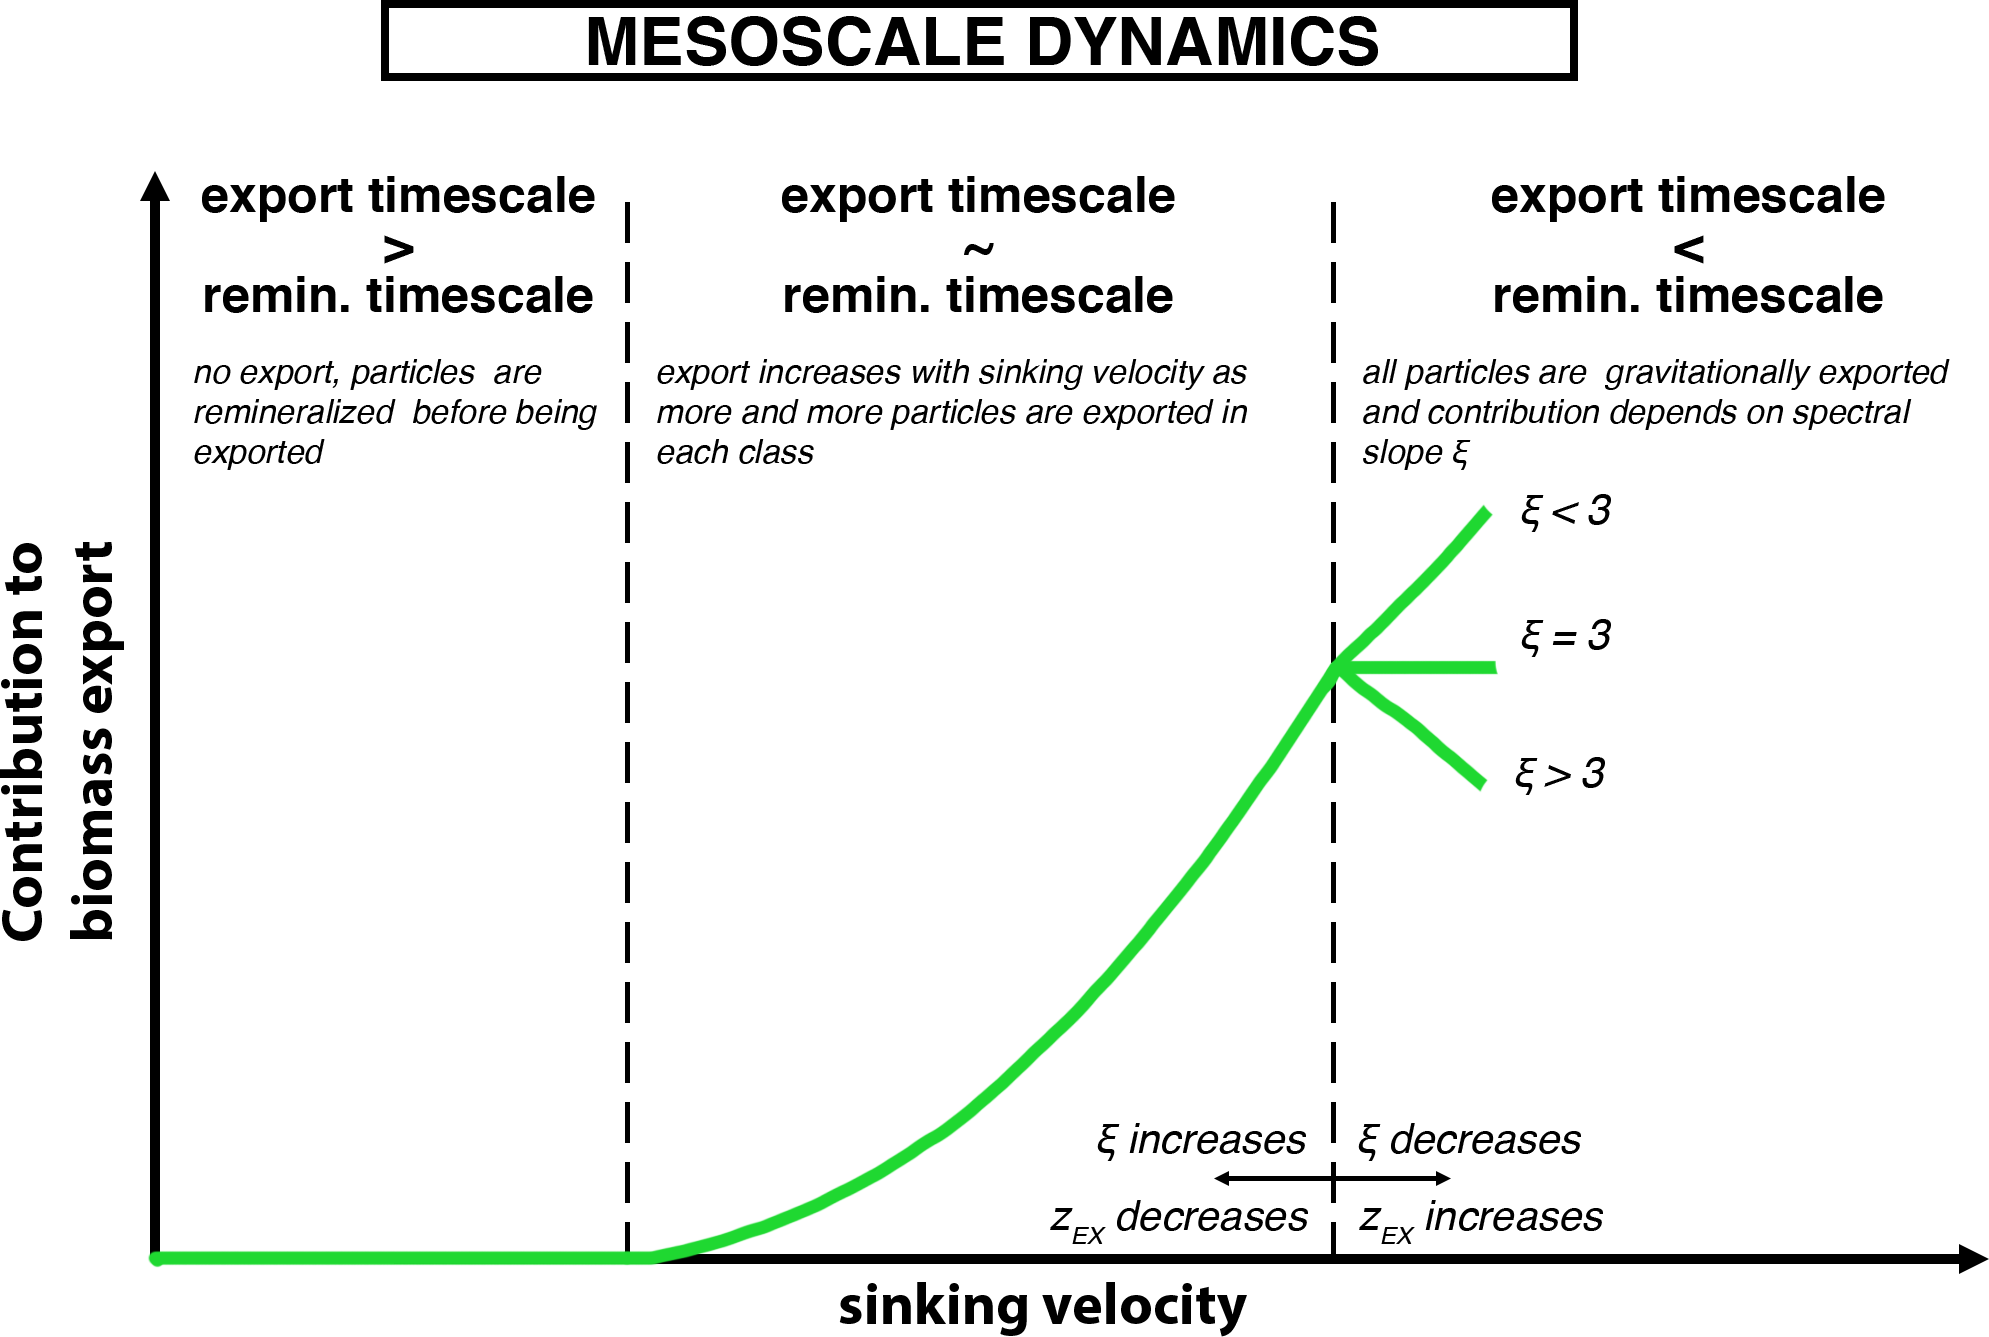
\includegraphics[width = .65\linewidth]{figures/cartoon_meso}\\[.2cm]
	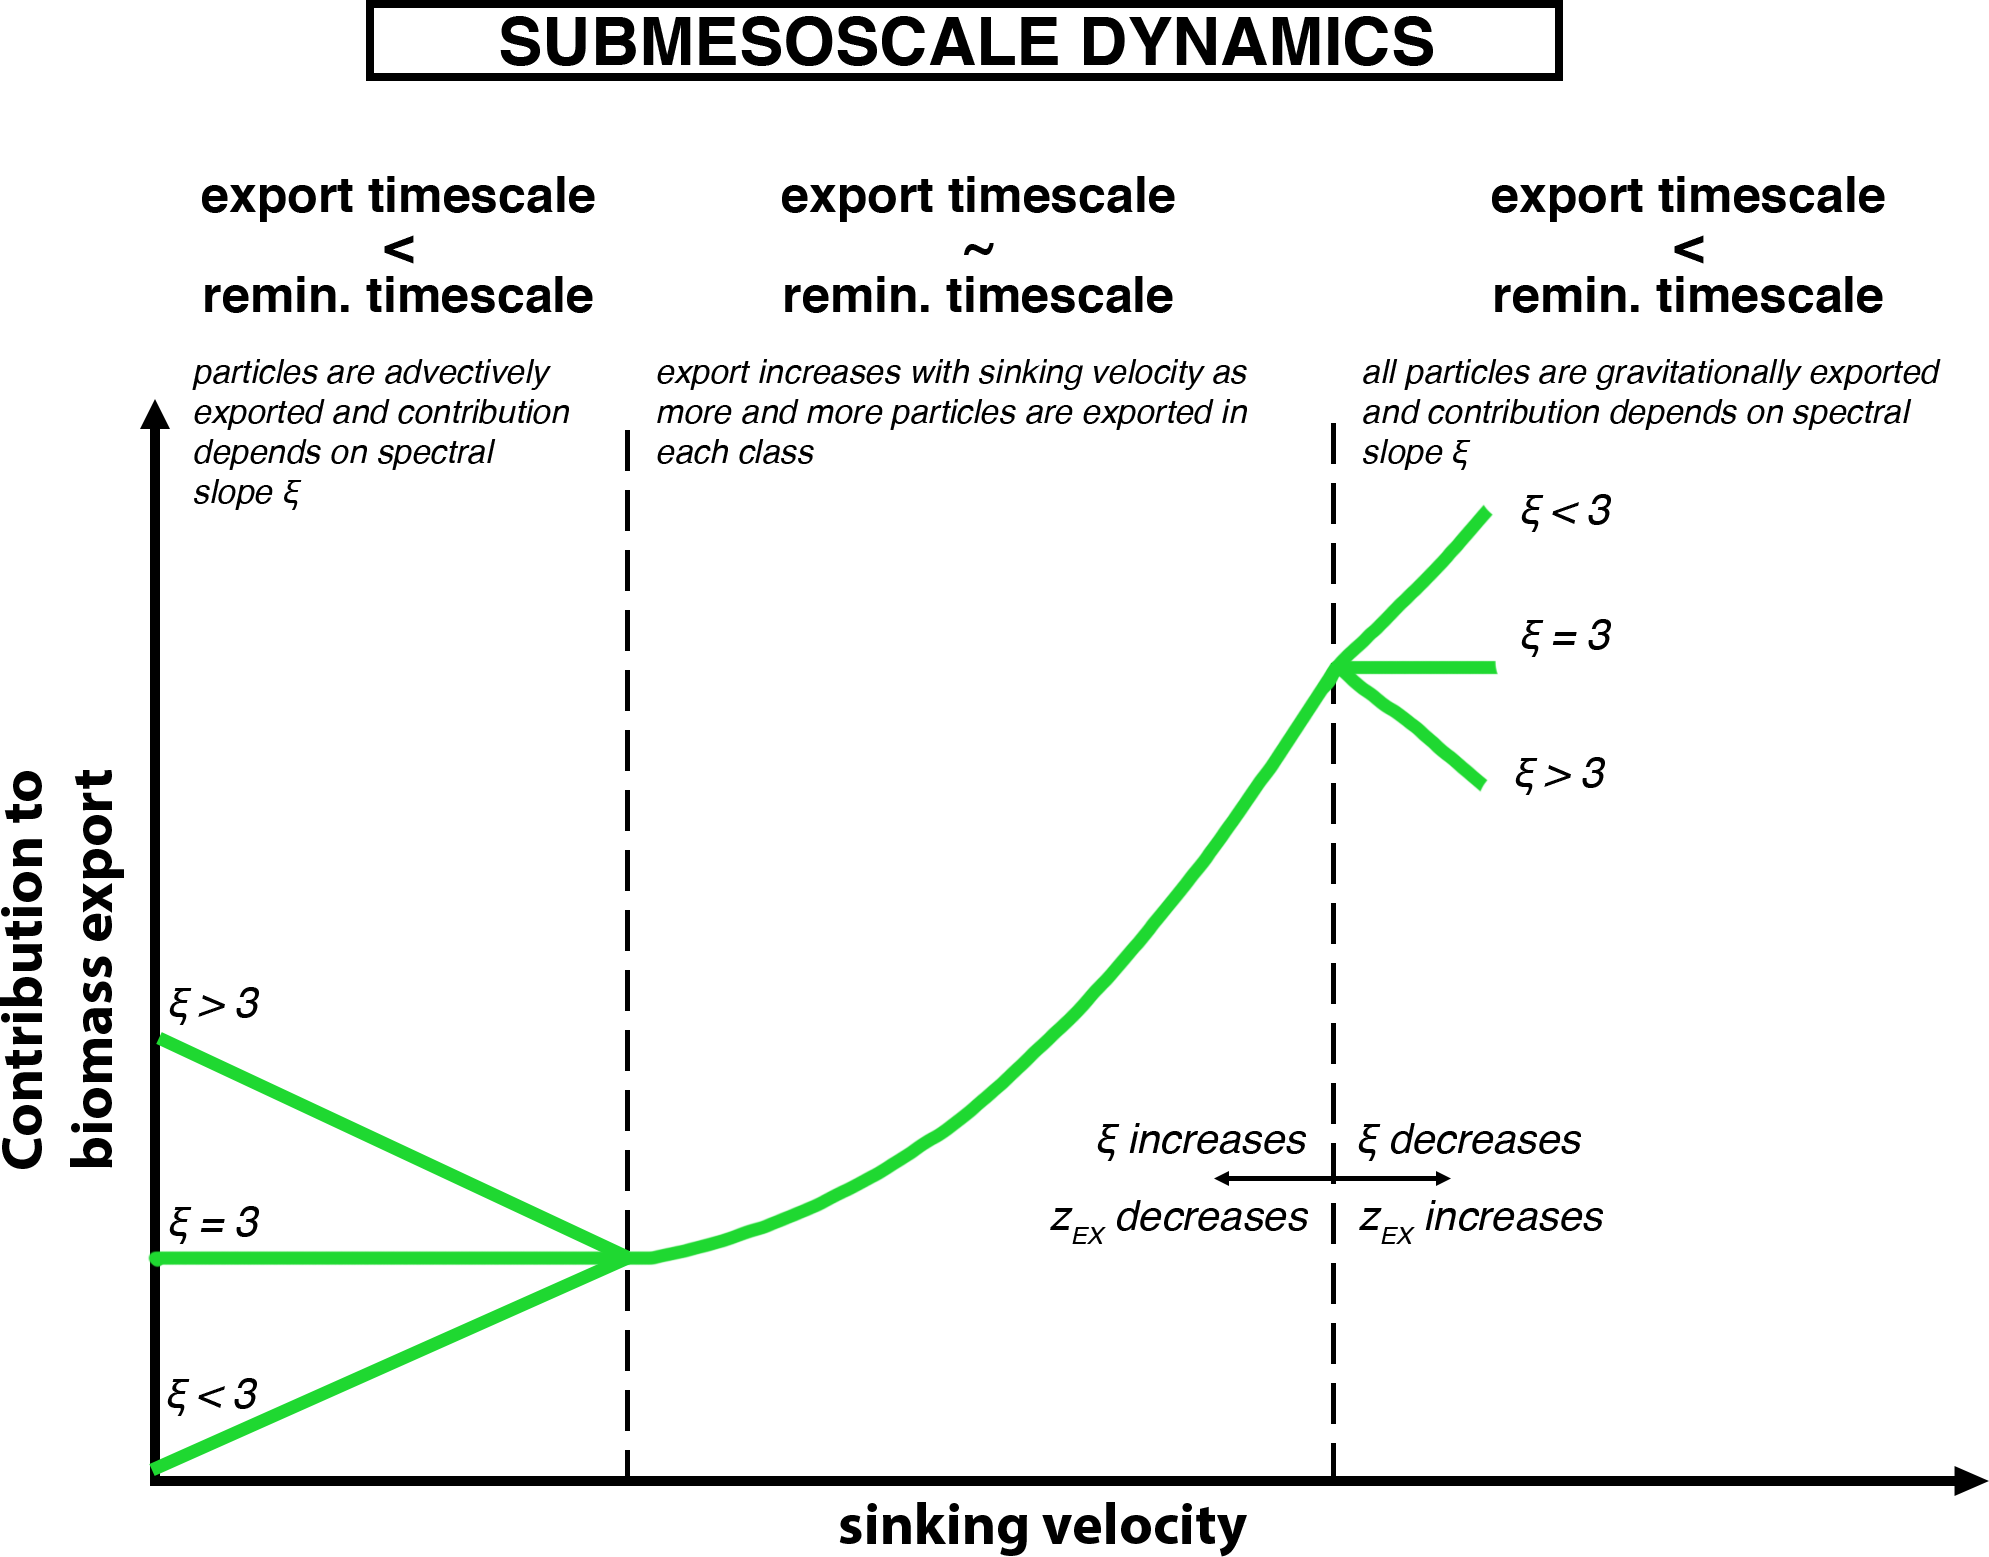
\includegraphics[width = .65\linewidth]{figures/cartoon_submeso}
	\caption{Schematics showing the respective contribution to export of particles with different sinking velocities in (top) a gravitationally-driven system (i.e., weak submesoscale dynamics), and (bottom) an advectively-driven system (i.e., strong submesoscale dynamics).}
	\label{fig: export_cartoon}
\end{figure}

In a system affected by submesoscale dynamics, localized strong downwelling vertical currents are generated. This effectively shortens the export timescale of slower-sinking particles, entering a regime where export timescales are shorter than remineralization timescales (Figure \ref{fig: export_cartoon}). In this regime, slower-sinking particles significantly contribute to POC export. In this study, sinking-velocity classes that did not contribute to POC export in a mesoscale regime, are found to contribute up to 30\% of POC export in the most extreme case, where $\xi =4$. Implementing remineralization process has little to no impact on the respective contributions of the different sinking-velocity classes as the impact of remineralization is smaller in advectively-driven export mechanism, as opposed to gravitationally-driven.

\section{Conclusion}
\label{sec: Conclusions}
The main conclusions of this study are: 
\begin{enumerate}
\item Submesoscale activity at station Papa is enhanced in the wintertime, leading to larger vertical velocities than in the summertime. The export mechanism in the winter is thus driven by advective sinking, as opposed to gravitational sinking in the summertime.
\item Submesoscale dynamics generally enhance export by increasing the contribution of slower-sinking particles to POC export by increasing the number of particle exported through advective sinking. The contribution of slower-sinking particles in ageostrophic flows is at least significant, and can be dominant in specific conditions.
\item Contribution of slower-sinking particles to POC export depends on the slope of the particle size spectra (i.e., Junge Slope), that controls the relative number of particles per size class. Three cases emerge in this study:
\begin{enumerate}
	\item If the Junge slope is smaller than 3, larger particles contribute most to export independently of flow dynamics, as there are no mechanism capable of selectively exporting slower-sinking particles.
	\item If the Junge slope equals 3, the respective contributions of the different size classes depend on the dynamical characteristics of the flow, as it influences the number of particles being exported. If 100\% of the particles is exported in all sinking classes, then each class contributes equally to POC export.
	\item If the Junge slope is greater than 3, ocean dynamics become the determining factor on which classes dominate: in a mostly geostrophic flow with weak vertical velocities, an intermediate sinking-velocity class will dominate POC export. In a flow with ageostrophic circulation leading to larger vertical velocities, slower sinking classes can potentially dominate export.
	\end{enumerate}
\item Remineralization processes reduce the contribution of slower-sinking particles when export dynamics are dominated by gravitational sinking (i.e., in a geostrophic flow). As flow dynamics become ageostrophic, advective sinking leads the export and remineralization processes have a limited impact.
%\item[(5)] Under specific conditions (large Junge slope and strongly ageostrophic flow), remineralization processes counter-intuitively enhance the role of slower-sinking (and non-sinking) particles to the point where export is dominated by these slow-sinking particles, therefore challenging the traditional paradigm of carbon export.
\end{enumerate}

%These conclusions demonstrate the importance of resolving a large portion of the particle size spectrum to properly quantify export, especially in dynamical regimes where strong ageostrophic circulation is present.

\section*{Acknowledgments}

The authors acknowledge support from the National Aeronautics and Space Administration as part of the EXport Processes in the global Ocean from RemoTe Sensing (EXPORTS) program - grant NNX16AR48G. We would like to thank A. Thompson (Caltech) for his useful comments and suggestions, N. Pelland (NOAA) and Charlie Eriksen (University of Washington) for sharing the glider data collected at Ocean Station Papa, as well as Sebastian Essink for his assistance in developing the particle-tracking code. All data used in this manuscript are publicly available: Ocean Station Papa data is available on PMEL's website (\url{https://www.pmel.noaa.gov/ocs/Papa}) and gridded ARGO products can be downloaded at \url{http://www.seanoe.org/data/00348/45945}. Glider data, model outputs, and particle trajectories are freely available on request. % Finally, we are grateful to the two anonymous reviewers for their valuable comments and suggestions.


%% ------------------------------------------------------------------------ %%
%%  REFERENCE LIST AND TEXT CITATIONS
%\bibliographystyle{apalike}
\bibliography{sinking_biblio}


%% ------------------------------------------------------------------------ %%
%
%  END ARTICLE
%
%% ------------------------------------------------------------------------ %%

%\end{article}
%\clearpage

%% ------------------------------------------------------------------------ %%
%
%  FIGURES AND TABLES
%
%% ------------------------------------------------------------------------ %%




%TAB2
%\begin{table}[]
%	\caption{Range of contributions (min-max) to the total amount of biomass exported per size class in both \textit{Papa\_summer} and \textit{Papa\_winter}.}
%	\label{tab: biomass_contribution}
%	\centering	
%	\begin{tabular}{|cc|c|c|c|c||c|c|c|c|}
%		\hline
%		&           & \multicolumn{4}{c||}{\textit{Papa\_summer}} & \multicolumn{4}{c|}{\textit{Papa\_winter}} \\
%		\hline
%		\multicolumn{2}{|c|}{sinking speed [m/day]} & 5               & 1             & 0.5          & 0.025     & 5              & 1            & 0.5          & 0.025       \\
%		\hline\hline
%		$\xi = 2$ & Remin OFF & 69-100\%     & 0-30\%     & 0-1\%     & 0\%       & 70-100\%    & 0-24\%    & 0-6\%     & 0\%         \\
%		\rowcolor[HTML]{EFEFEF} 
%		 & Remin ON  & 100\%           & 0\%           & 0\%          & 0\%       & 92-100\%    & 0-6\%     & 0-3\%     & 0-1\%    \\
%		$\xi = 3$ & Remin OFF & 49-100\%     & 0-49\%     & 0-2\%     & 0\%       & 49-100\%    & 0-37\%    & 0-12\%    & 0-3\%    \\
%		\rowcolor[HTML]{EFEFEF} 
%		& Remin ON  & 100\%           & 0\%           & 0\%          & 0\%       & 78-100\%    & 0-11\%    & 0-9\%     & 0-6\%    \\
%		$\xi = 4$ & Remin OFF & 30-100\%     & 0-68\%     & 0-3\%     & 0\%       & 25-99\%     & 0-43\%    & 0-20\%    & 0-25\%   \\
%		\rowcolor[HTML]{EFEFEF} 
%		& Remin ON  & 100\%           & 0\%           & 0\%          & 0\%       & 38-100\%    & 0-16\%    & 0-14\%    & 0-39\%  \\ 
%		\hline
%	\end{tabular}
%\end{table}
\end{document}

%%%%%%%%%%%%%%%%%%%
%%%% OBSOLETE %%%%%
%%%%%%%%%%%%%%%%%%%
The main consequence of this result is that, when the biomass spectrum has a negative slope (i.e., $\xi>3$) , 



It is impossible to obtain $N_{slow} > N_{fast}$


In the absence of remineralization,
 
In a gravitationally-driven system (i.e., weak submesoscale activity), contribution to export generally increases as sinking-velocity increases. This is true up to the point where the totality of the particles are exported: for an equal number of particle exported, the 

Generally, export is dominated by the contribution of faster-sinking particles. For a slower-sinking velocity class to contribute more to the export than a faster-sinking velocity class, the number of particles exported must satisfy:



In the absence of remineralization, where all particles are eventually exported, this condition is only satisfied if $\xi>3$, that is if the biomass spectrum has a negative slope (see Figure \ref{fig: sinking_velocity_spectrum}). \fixme{While export will then always be dominated by faster-sinking particles, the contribution of slower-sinking particles varies greatly with the 
as a function of (1) the biomass spectral slope must be negative (i.e., $\xi>3$), and (2) the number of particles exported must be large enough. The number of particles to be exported for a slower-sinking velocity class to dominate export over a faster-sinking velocity class depend on the Junge slope and is determined by:
Under those conditions, the contribution to export as a function of sinking speed is notc linear: increasingly faster-sinking classes contribute increasingly to export, as they physically export more particles, until the sinking speed above which 100\% of the particles are exported is reached. Above this threshold, the contribution to biomass export by increasingly faster-sinking particles decreasingly contribute to export, due to the negative slope in the biomass spectra. Despite the export being dominated by faster-sinking particles, this study demonstrates that in the presence of submesoscale activity, slower-sinking particles have the potential to significantly contribute to the total export. The slowest sinking-velocity class simulated in this study contributed to up to 13\% of the total biomass export in the presence of submesoscale dynamics, for $\xi = 4$.}

The important threshold in the Junge slope highlighted in this study can be generally defined by the log-log slope between particle size and biomass content. In this study, we assume that biomass varies as the volume of the particle (B $\propto r^3$), thus obtaining a threshold of $\xi=3$. Using other relationships between biomass and particle size will not impact the main conclusions of this study, but will only affect the threshold at which slower-sinking particles contribute significantly to the export.

\subsection{Impacts of  Particle Remineralization}
\label{sec: discuss_remin}

Remineralization processes introduce a time-dependency in the relationship between biomass and sinking-velocity. A simple, yet commonly-used, remineralization scheme was imposed to the particles. As one would expect, the main impacts of implementing a remineralization scheme is a decrease in the exported biomass across all sinking-velocity classes, as well as a prolonged export timescale. This is due to the fact that, as a particle remineralizes, its sinking-velocity decreases. Because the particle now takes more time to be exported, it further remineralizes, which in turn decreases the particle's sinking-velocity. In the summer, this self-reinforcing mechanism affects slower-sinking classes the most, and therefore significantly decreases their contribution to export. In the winter, remineralization also generally reduces the amount of biomass exported, although the impact is far less pronounced and affects all sinking-velocity classes similarly. This is explained by the different mechanism dominating export in the summer and winter: In the summertime, export is dominated by gravitational sinking, which is directly impacted by remineralization processes. In the wintertime, however, export is largely driven by advective sinking through the stronger downward currents observed in the submesoscale flow. Advective sinking being independent from remineralization processes, the biomass export is less affected than in the summertime. In fact, our analysis clearly shows that remineralization processes does not significantly impact the biomass export associated with slower-sinking velocity classes over the first 5 days of the simulations. 

Finally, a very interesting feature arose from implementing a remineralization scheme to the Lagrangian particles. In the winter and with $\xi =4$, the biomass exported by the slowest-sinking class (0.025 m/day) consistently exceeds the amount of biomass exported by slightly faster-sinking classes (0.5 and 1 m/day), despite a considerably smaller number of particles exported ($<4$\% vs. 23\% and 73\%, respectively) This non-intuitive result emerges from the exponential characteristic of the remineralization scheme: the impact of remineralization thus increases with the sinking velocity. This result demonstrates that remineralization can, under specific circumstances, increase the role played by slower sinking-velocity classes. The necessary conditions involve a large Junge slope and strong submesoscale activity.
